\chapter{Three Dimensional High Dynamic Range for 3D Range-Sensing Cameras}
\label{3dhdr3dsensing}

%\section{Abstract}
This chapter presents the invention and implementation of Three Dimensional High Dynamic Range 
(3DHDR) sensing, along with examples. A method for 3DHDR veillance (sensing, computer vision, 
and video capture) by integrating tonal and spatial information obtained from multiple HDR exposures 
was proposed for the use in conjunction with one or more 3D (range sensing) cameras.

In one embodiment, a 3DHDR camera setup from multiple 3D cameras such as the Microsoft Kinect 
system was constructed, where the 3D cameras were arranged in a fixed rig such that the calibration 
parameters between the cameras remain constant over time. With the proposed setup, only a single 
automated camera calibration step is required at the initial time of assembling and fixing the cameras 
into the array.  Preferably, the cameras either view from the same position through beam splitters, or 
are fixed close to one another, so that they capture approximately the same subject matter. The 
system is designed so the cameras each capture a differently exposed image or video of 
approximately the same subject matter.  In one embodiment, two Kinect cameras are attached 
together facing in the same direction, with a neutral density (ND) filter over one of them to obtain a 
darker exposure.  The dark and light exposures are combined to obtain more accurate 3D sensing in 
high contrast scenes.  In another embodiment, a single 3D camera is exposure-sequenced 
(alternating light and dark exposures) to further simplify the setup.

3DHDR might, more generally, be incorporated into existing 3D cameras, resulting in a new kind of 3D 
sensor that can work in nearly any environment, including high contrast scenes such as outdoor 
scenes, or scenes where a variable range is needed.

\subsection{High Dynamic Range Imaging with Range Sensing Camera}
HDR (High Dynamic Range) has been a well-known and well-studied field of
research for 20 years.  As Roberston et al. reported:
\begin{quote}
``The first report of digitally combining multiple pictures
 of the same scene to improve dynamic range appears to be
 Mann~\cite{mannist}.
 Algorithmic detail that is lacking from Ref.~\cite{mannist} is
 provided in a later publication,~\cite{mannwyckofftr}
 where Mann and Picard explicitly examine the situation where multiple pictures,
 each of different exposures, are taken of a scene. They
 provide a method of merging these multiple exposures to
 form a single image with an effective dynamic range
 greater than that of the camera. By making use of certainty
 functions, which give a measure of the confidence in an
 observation, Mann and Picard weight the observations from
 the various exposures to provide the final image. The certainty
 function for a particular camera is computed as the
 derivative of the camera response function, which results in
 low confidence for pixel values near extremes, and higher
 confidence for pixel values
 between these extremes.''~\cite{robertson2003estimation}
\end{quote}

HDR photography~\cite{candocia1, candocia2, candocia3, wyckoff1962experimental, 
mannist} and video~\cite{mann2012hdrchitecture,lo2012high,mann2012realtime, 
HDRVideoCamera11, kang2003high} are attractive topics as they address one of the most 
fundamental problems of digital camera sensors namely their limited dynamic range.

Moreover, HDR is not limited to being only applicable to color cameras, but it can also be applied to 
cameras that operate outside the visible spectrum, such as infrared cameras, as well as to 3D 
cameras.  The light capturing mechanism of cameras, whether it be analog (film) or digital (CMOS/
CCD sensors), can only record a limited range of information from any scene. Combining 
differently exposed images of the same scene can produce an image of higher range than any of 
the individual images used to create it. The invention of the infrared (IR) 3D camera proposed in 
this chapter brings forth the added spatial dimension and extends the spectral range that can be 
captured. Using both a visual light camera and an IR-3D camera allows the capture of an additional 
spatial dimension and extended spectral range. Applying HDR photography techniques to such a 
combined system not only increases the dynamic range of the visual camera but possibly also the 
range of the additional spatial dimension (e.g. making 3D cameras useful outdoors in bright 
sunlight or in high contrast scenes where glare from bare light bulbs might otherwise degrade the 
3D data, or improving the range of the sensor in both long and short distance range).

%Simultaneously on colour and infrared-3D (IR-3D) camera, on a Microsoft Kinect, and thus 
%increases the visual range from the colour cameras and the depth range of the IR-3D camera. 

\subsection{Conventional uses of Kinect: Motion Sensing and Surveillance}
The Kinect system, from Microsoft, was designed to capture motion with the Microsoft Xbox 360 
gaming console.  The Kinect system allows the gamer to interact with games without the need for 
physical controllers. It accomplishes this by tracking the user's movements and position in 3-D 
space, with respect to itself, in real-time. In normal use, the Kinect system is stationary and 
observes the gamer as he/she moves.  In this sense, the Kinect system was envisioned and 
created as a surveillance camera (i.e., to be borne by inanimate objects rather than to be worn). 

%%\begin{figure*}[!t]
%%\centering
%%\subfloat[Top]{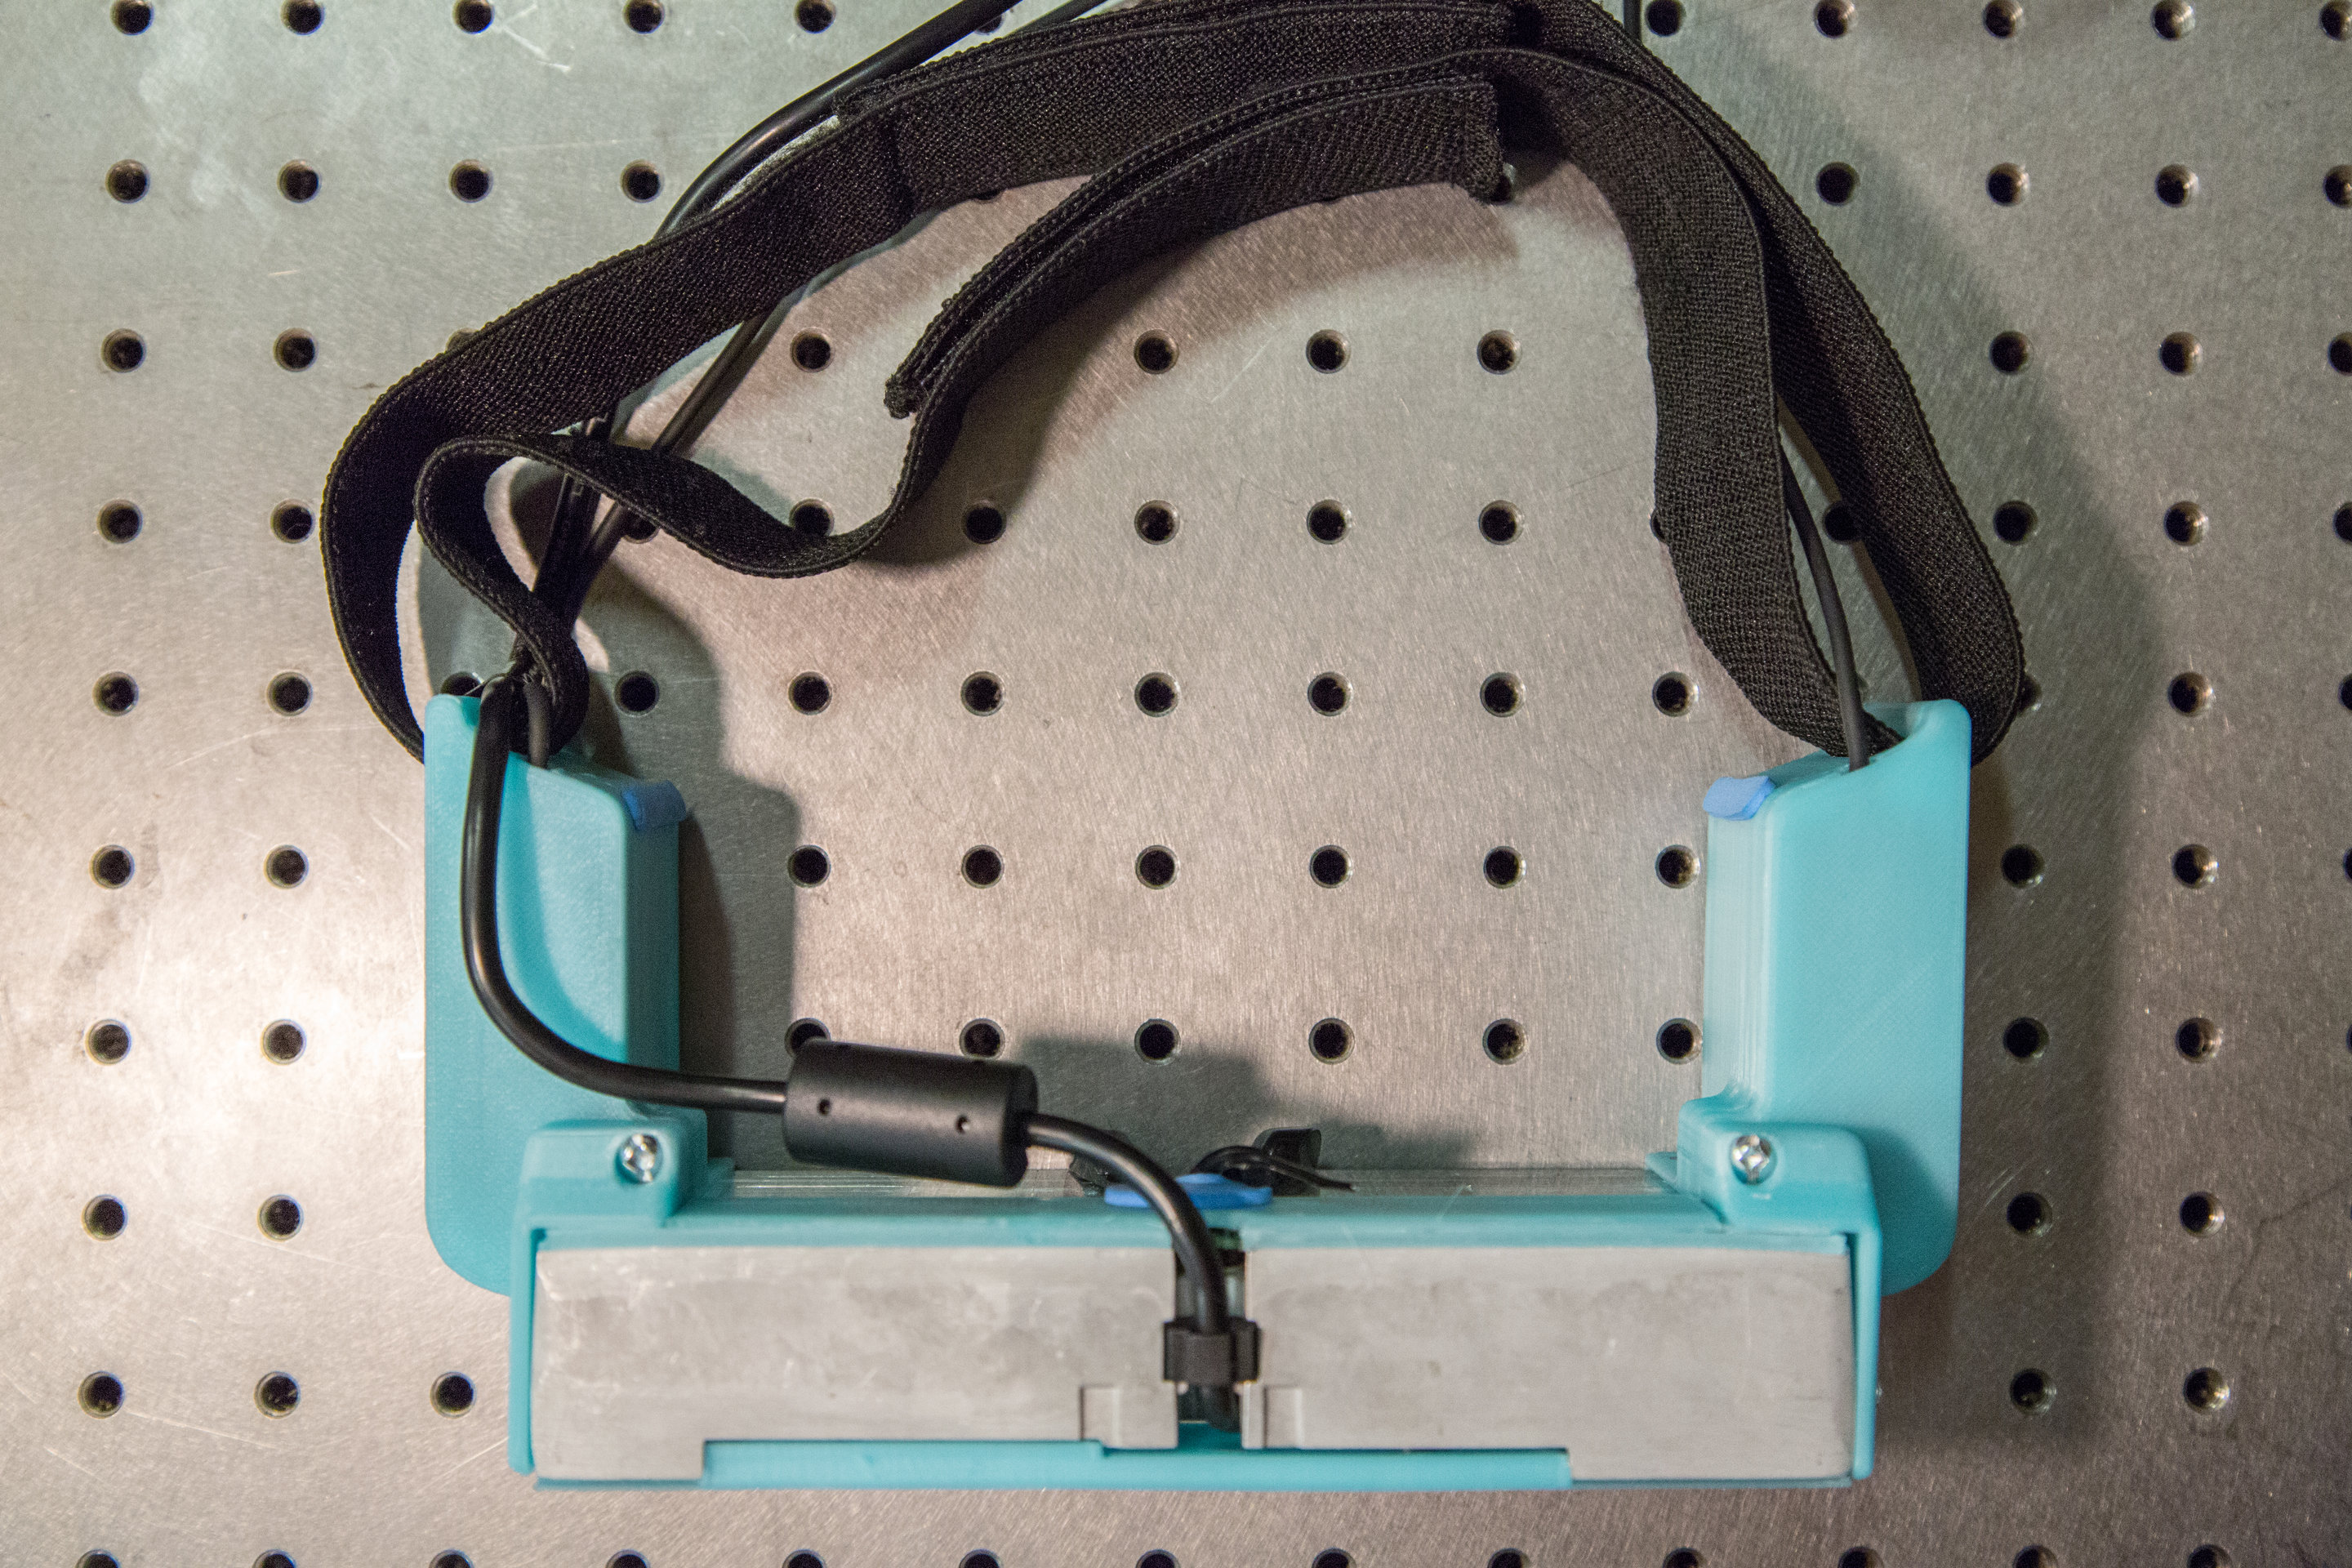
\includegraphics[height=1.4in]{ch4/diagrams/hdrglass/lowres/IMG_0257.jpg}
%%\label{fig_third_case}}
%%\subfloat[Front]{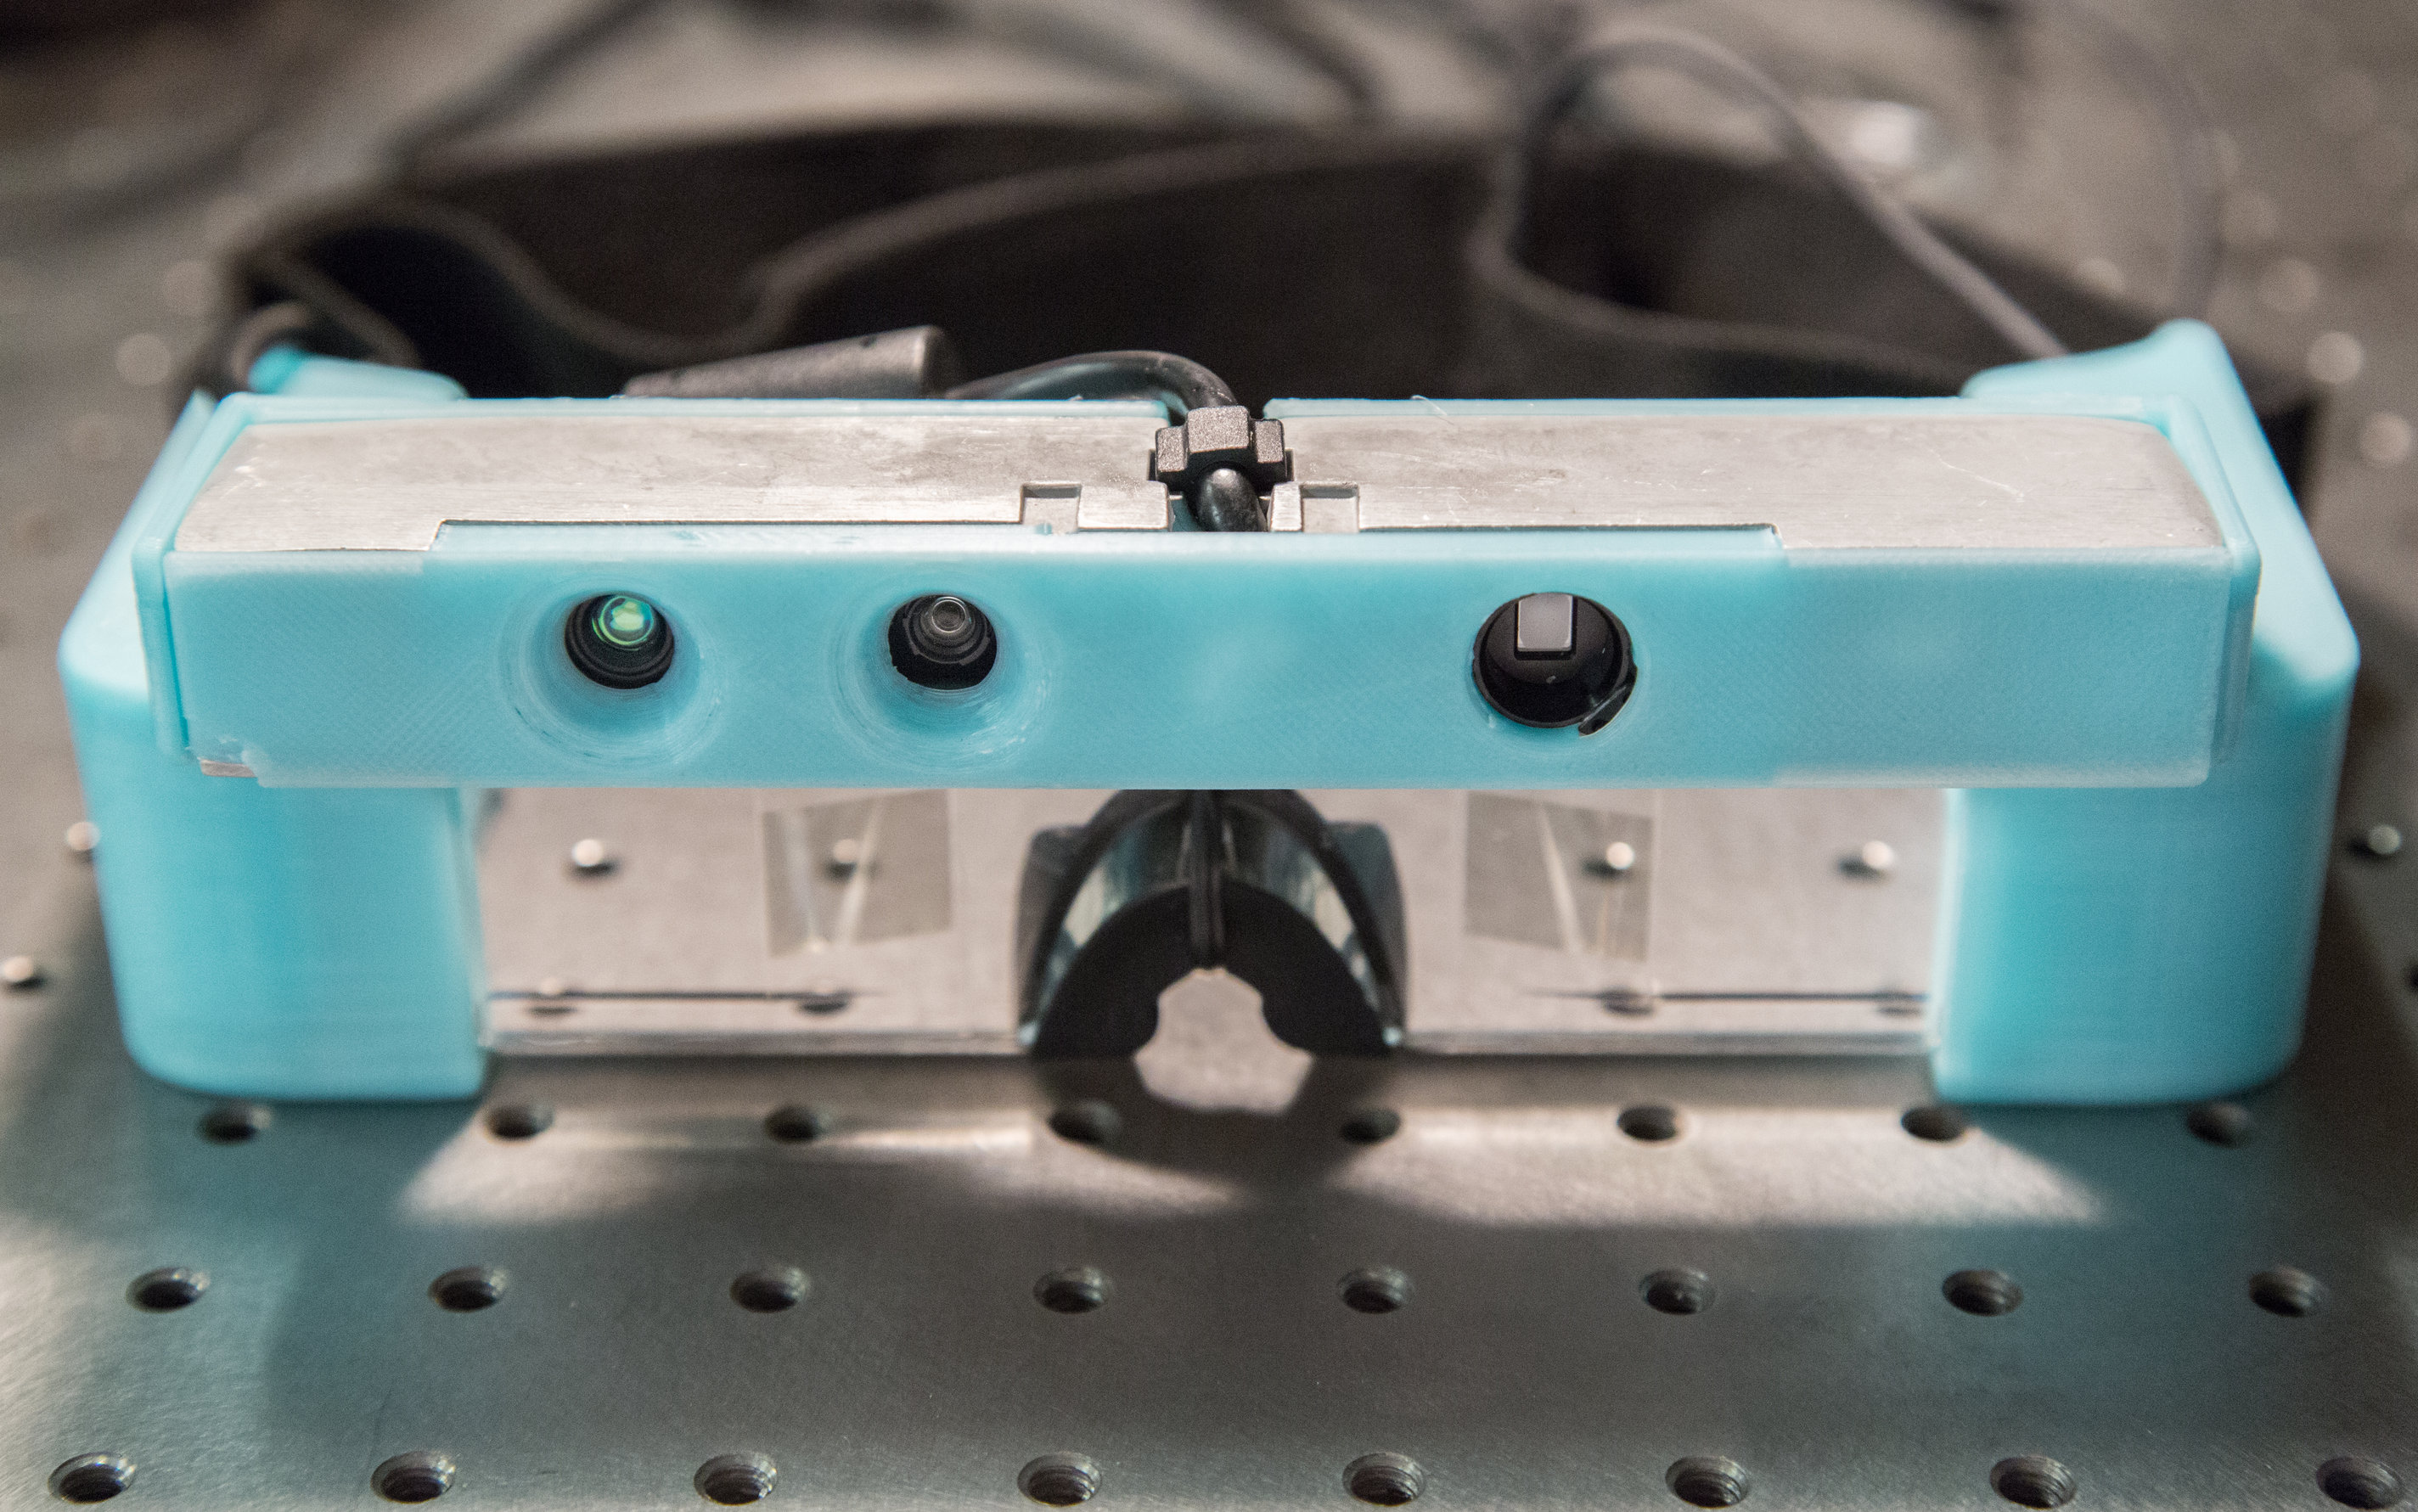
\includegraphics[height=1.4in]{ch4/diagrams/hdrglass/lowres/IMG_0263.jpg}
%%\label{fig_second_case}}
%%\subfloat[Side]{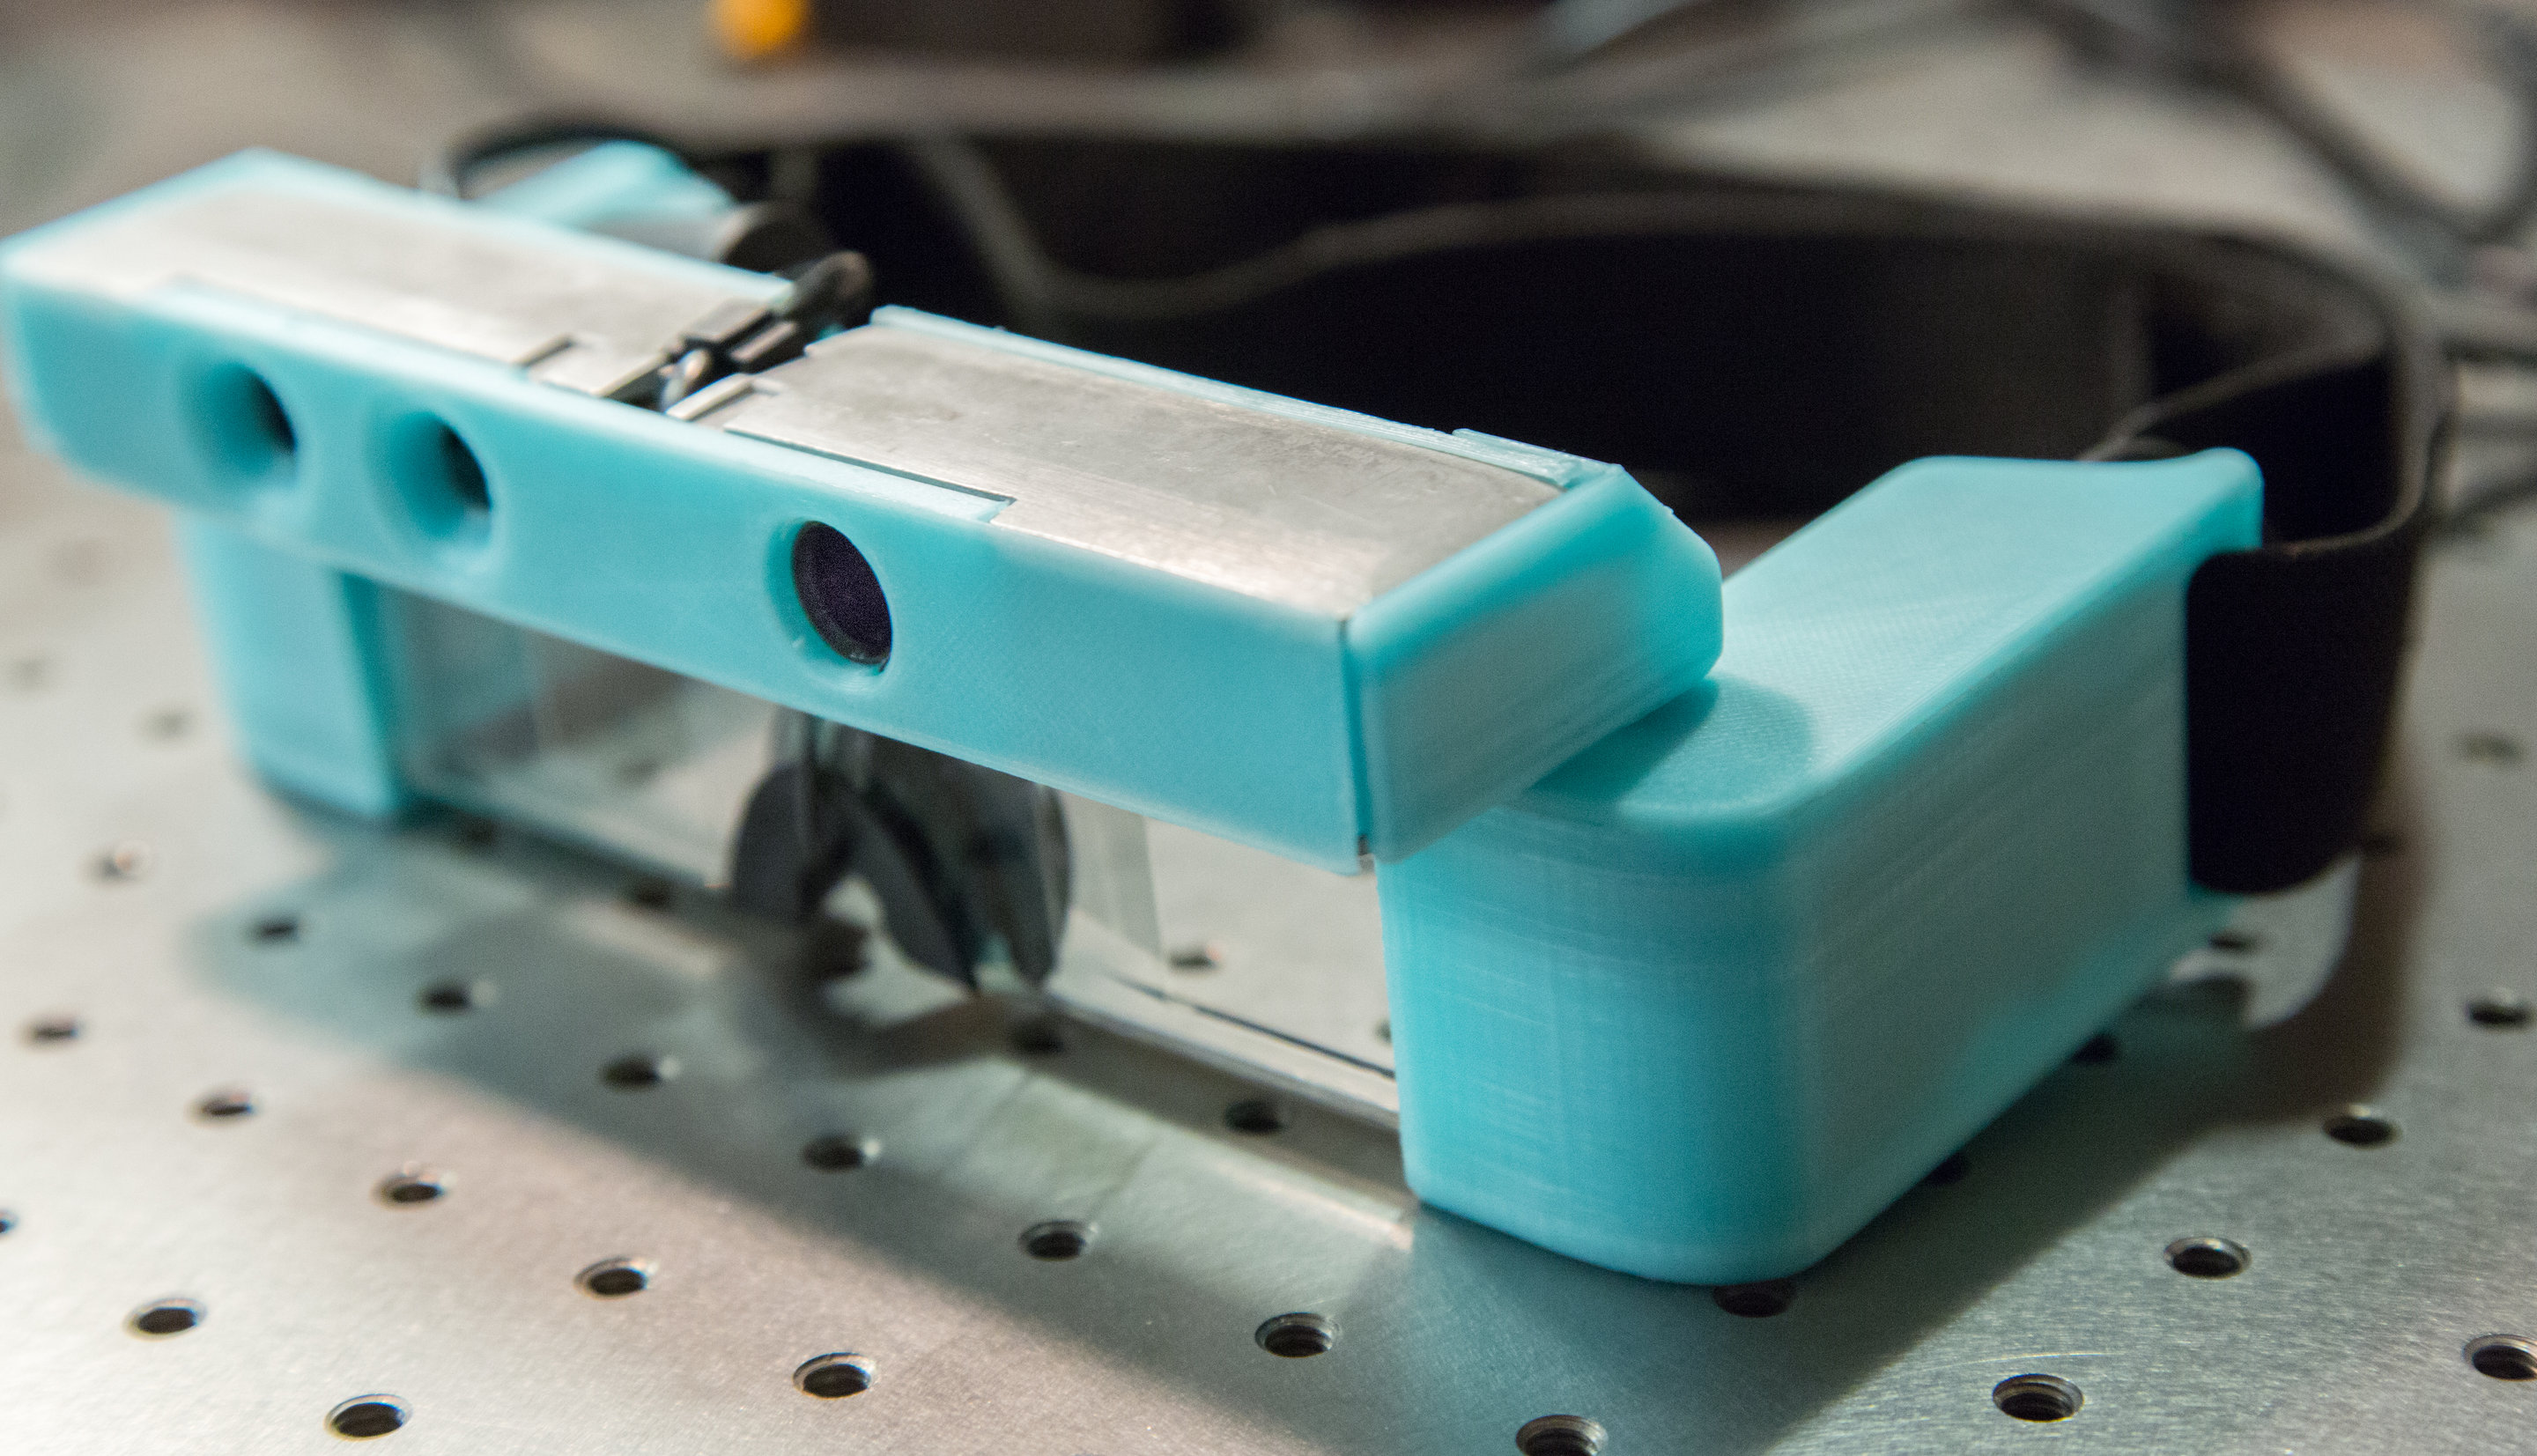
\includegraphics[height=1.4in]{ch4/diagrams/hdrglass/lowres/IMG_0258.jpg}
%%\label{fig_first_case}}
%%%\caption{Wearable Digital Eye Glass Prototype. Our custom 3D printed design allows users to 
%wear the digital glass in everyday life. The proposed algorithm can be utilized for improving the 
%dynamic range of the camera and thus allowing the users to see `better' in daily life. Notice that our 
%proposed system not only allows users to see in high contract scene, it also enables night vision due 
%to the use of active depth sensor which projects IR light patterns and reconstruct 3D information about 
%the scene. These provides users the ability to see in extreme environments, and also allows for robust 
%tracking algorithm to be integrated with the eyeglasses.}
%%\label{fig_wearable_glass}
%%\end{figure*}

\begin{figure*}
\centering
\begin{subfigure}{.32\textwidth}
\centering
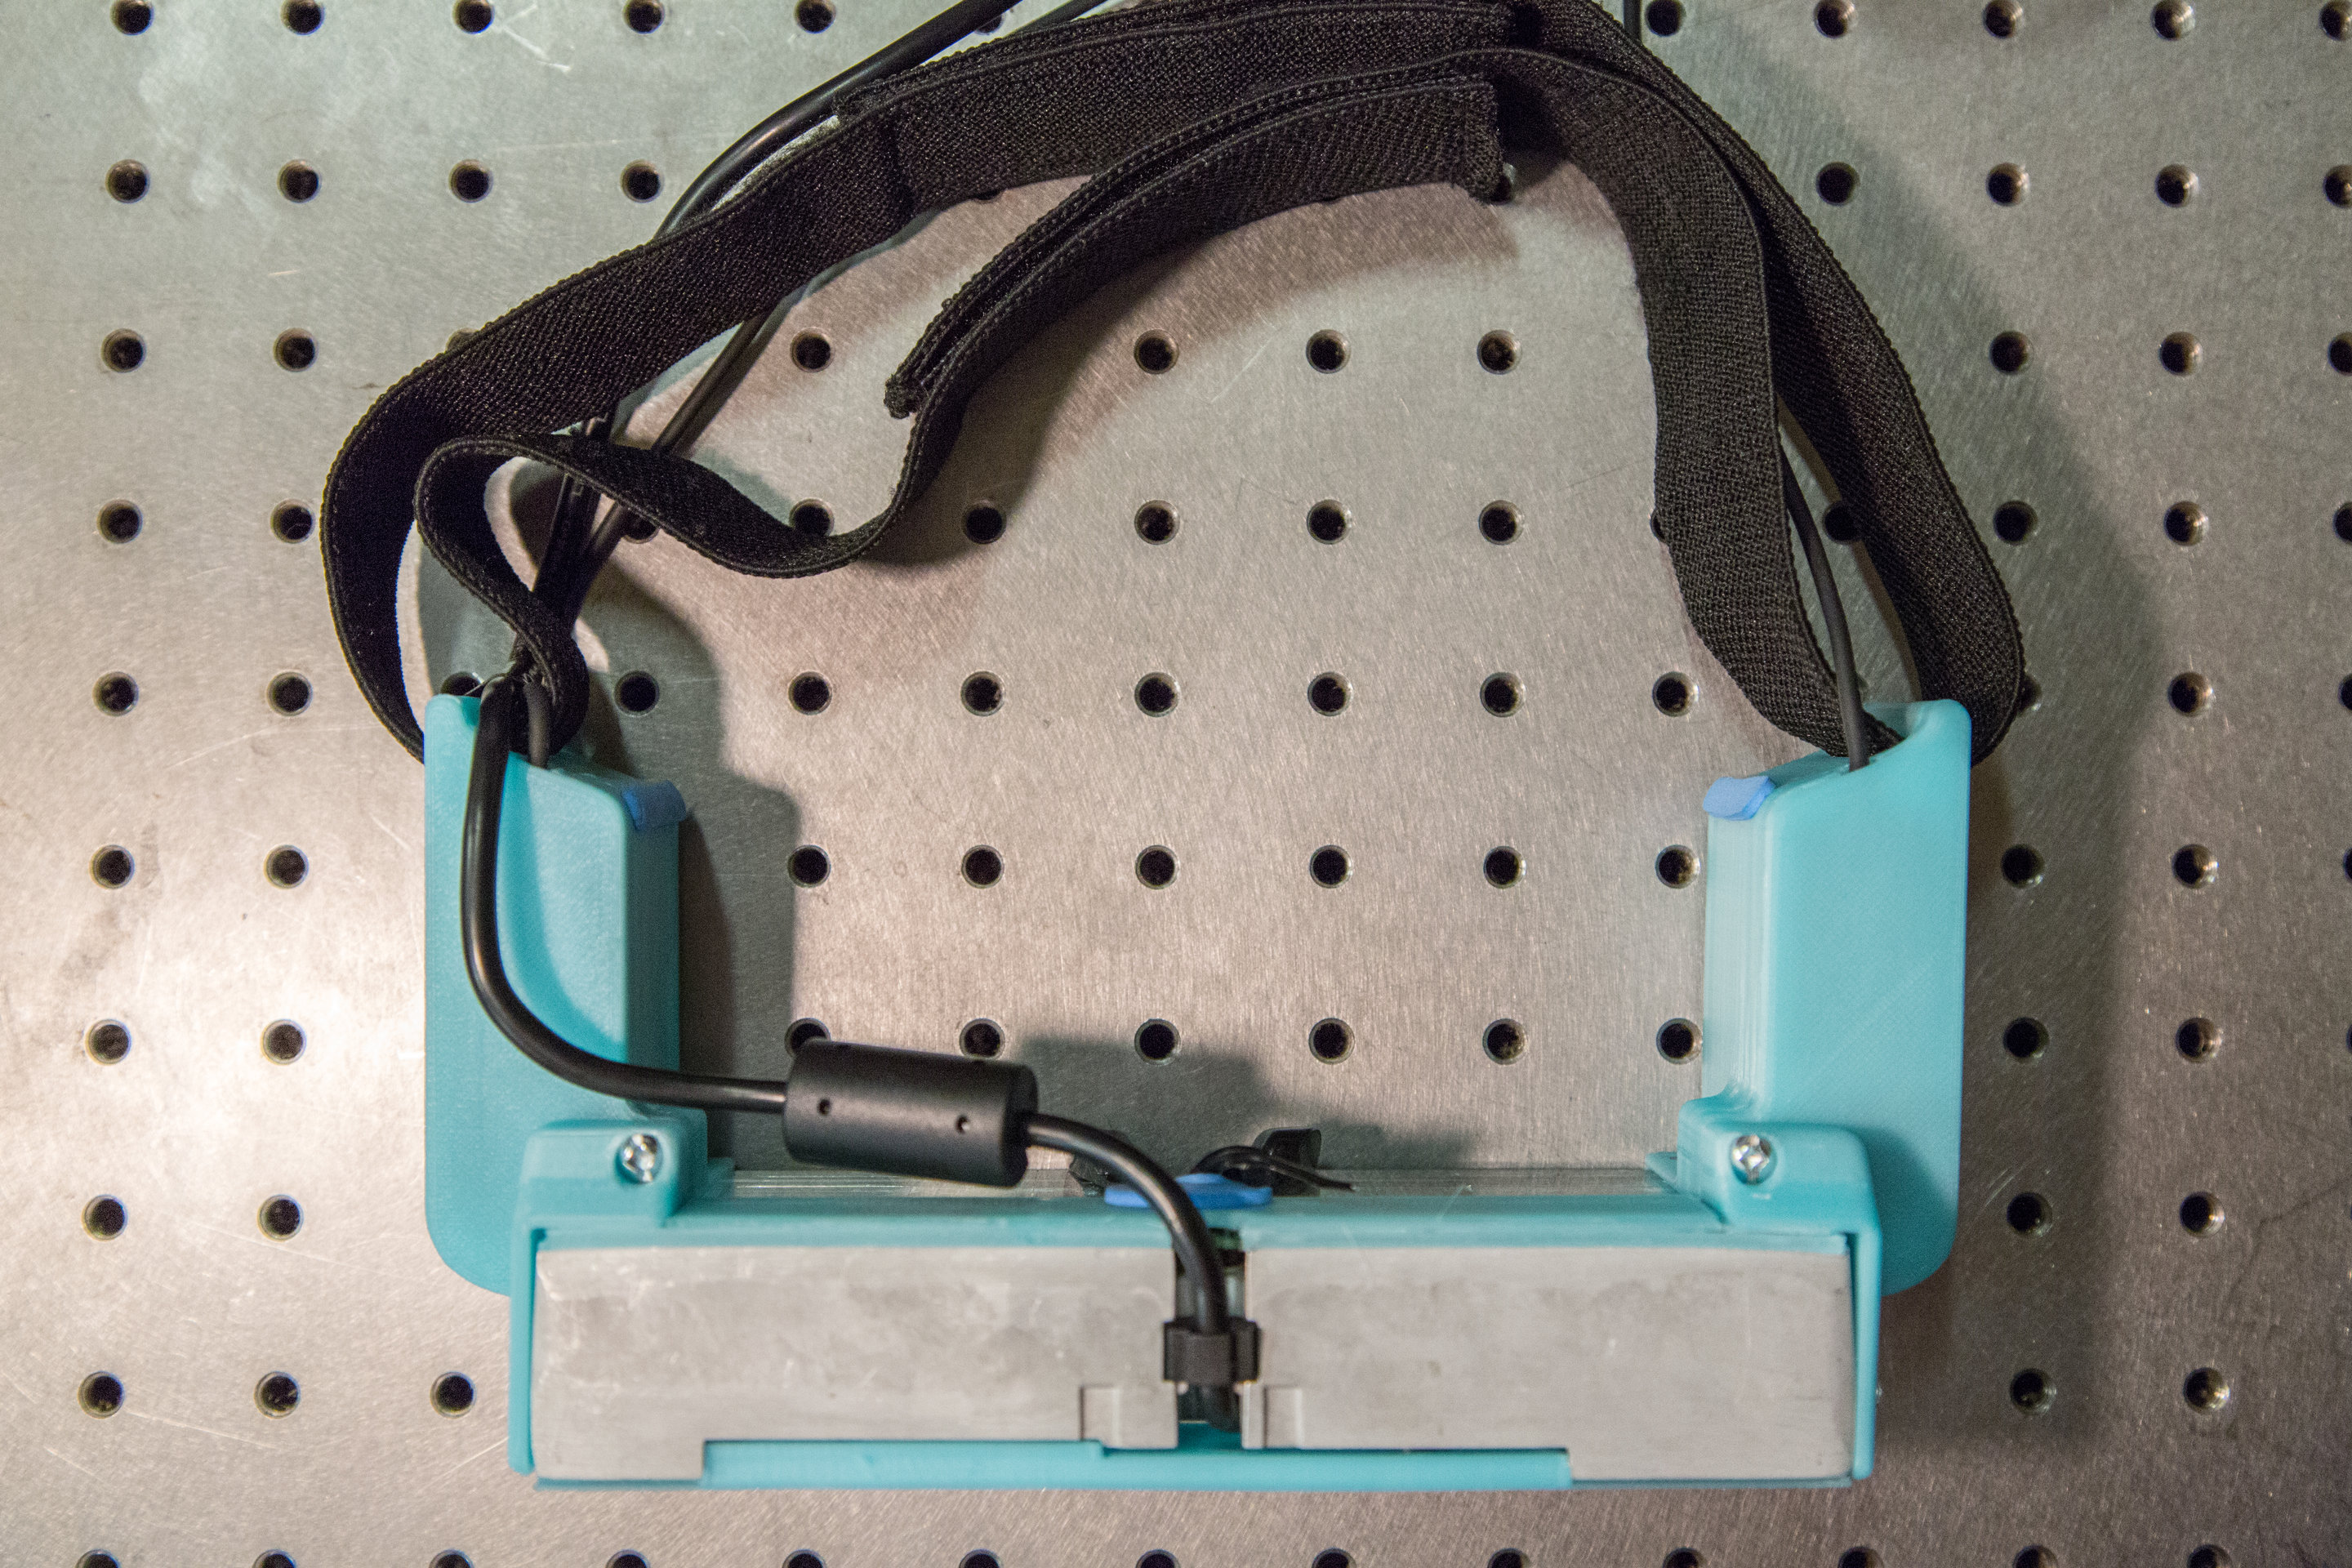
\includegraphics[height=1.2in]{ch4/diagrams/hdrglass/lowres/IMG_0257.jpg}
\caption{Top View}
\label{fig_third_case}
\end{subfigure}
~
\begin{subfigure}{.32\textwidth}
\centering
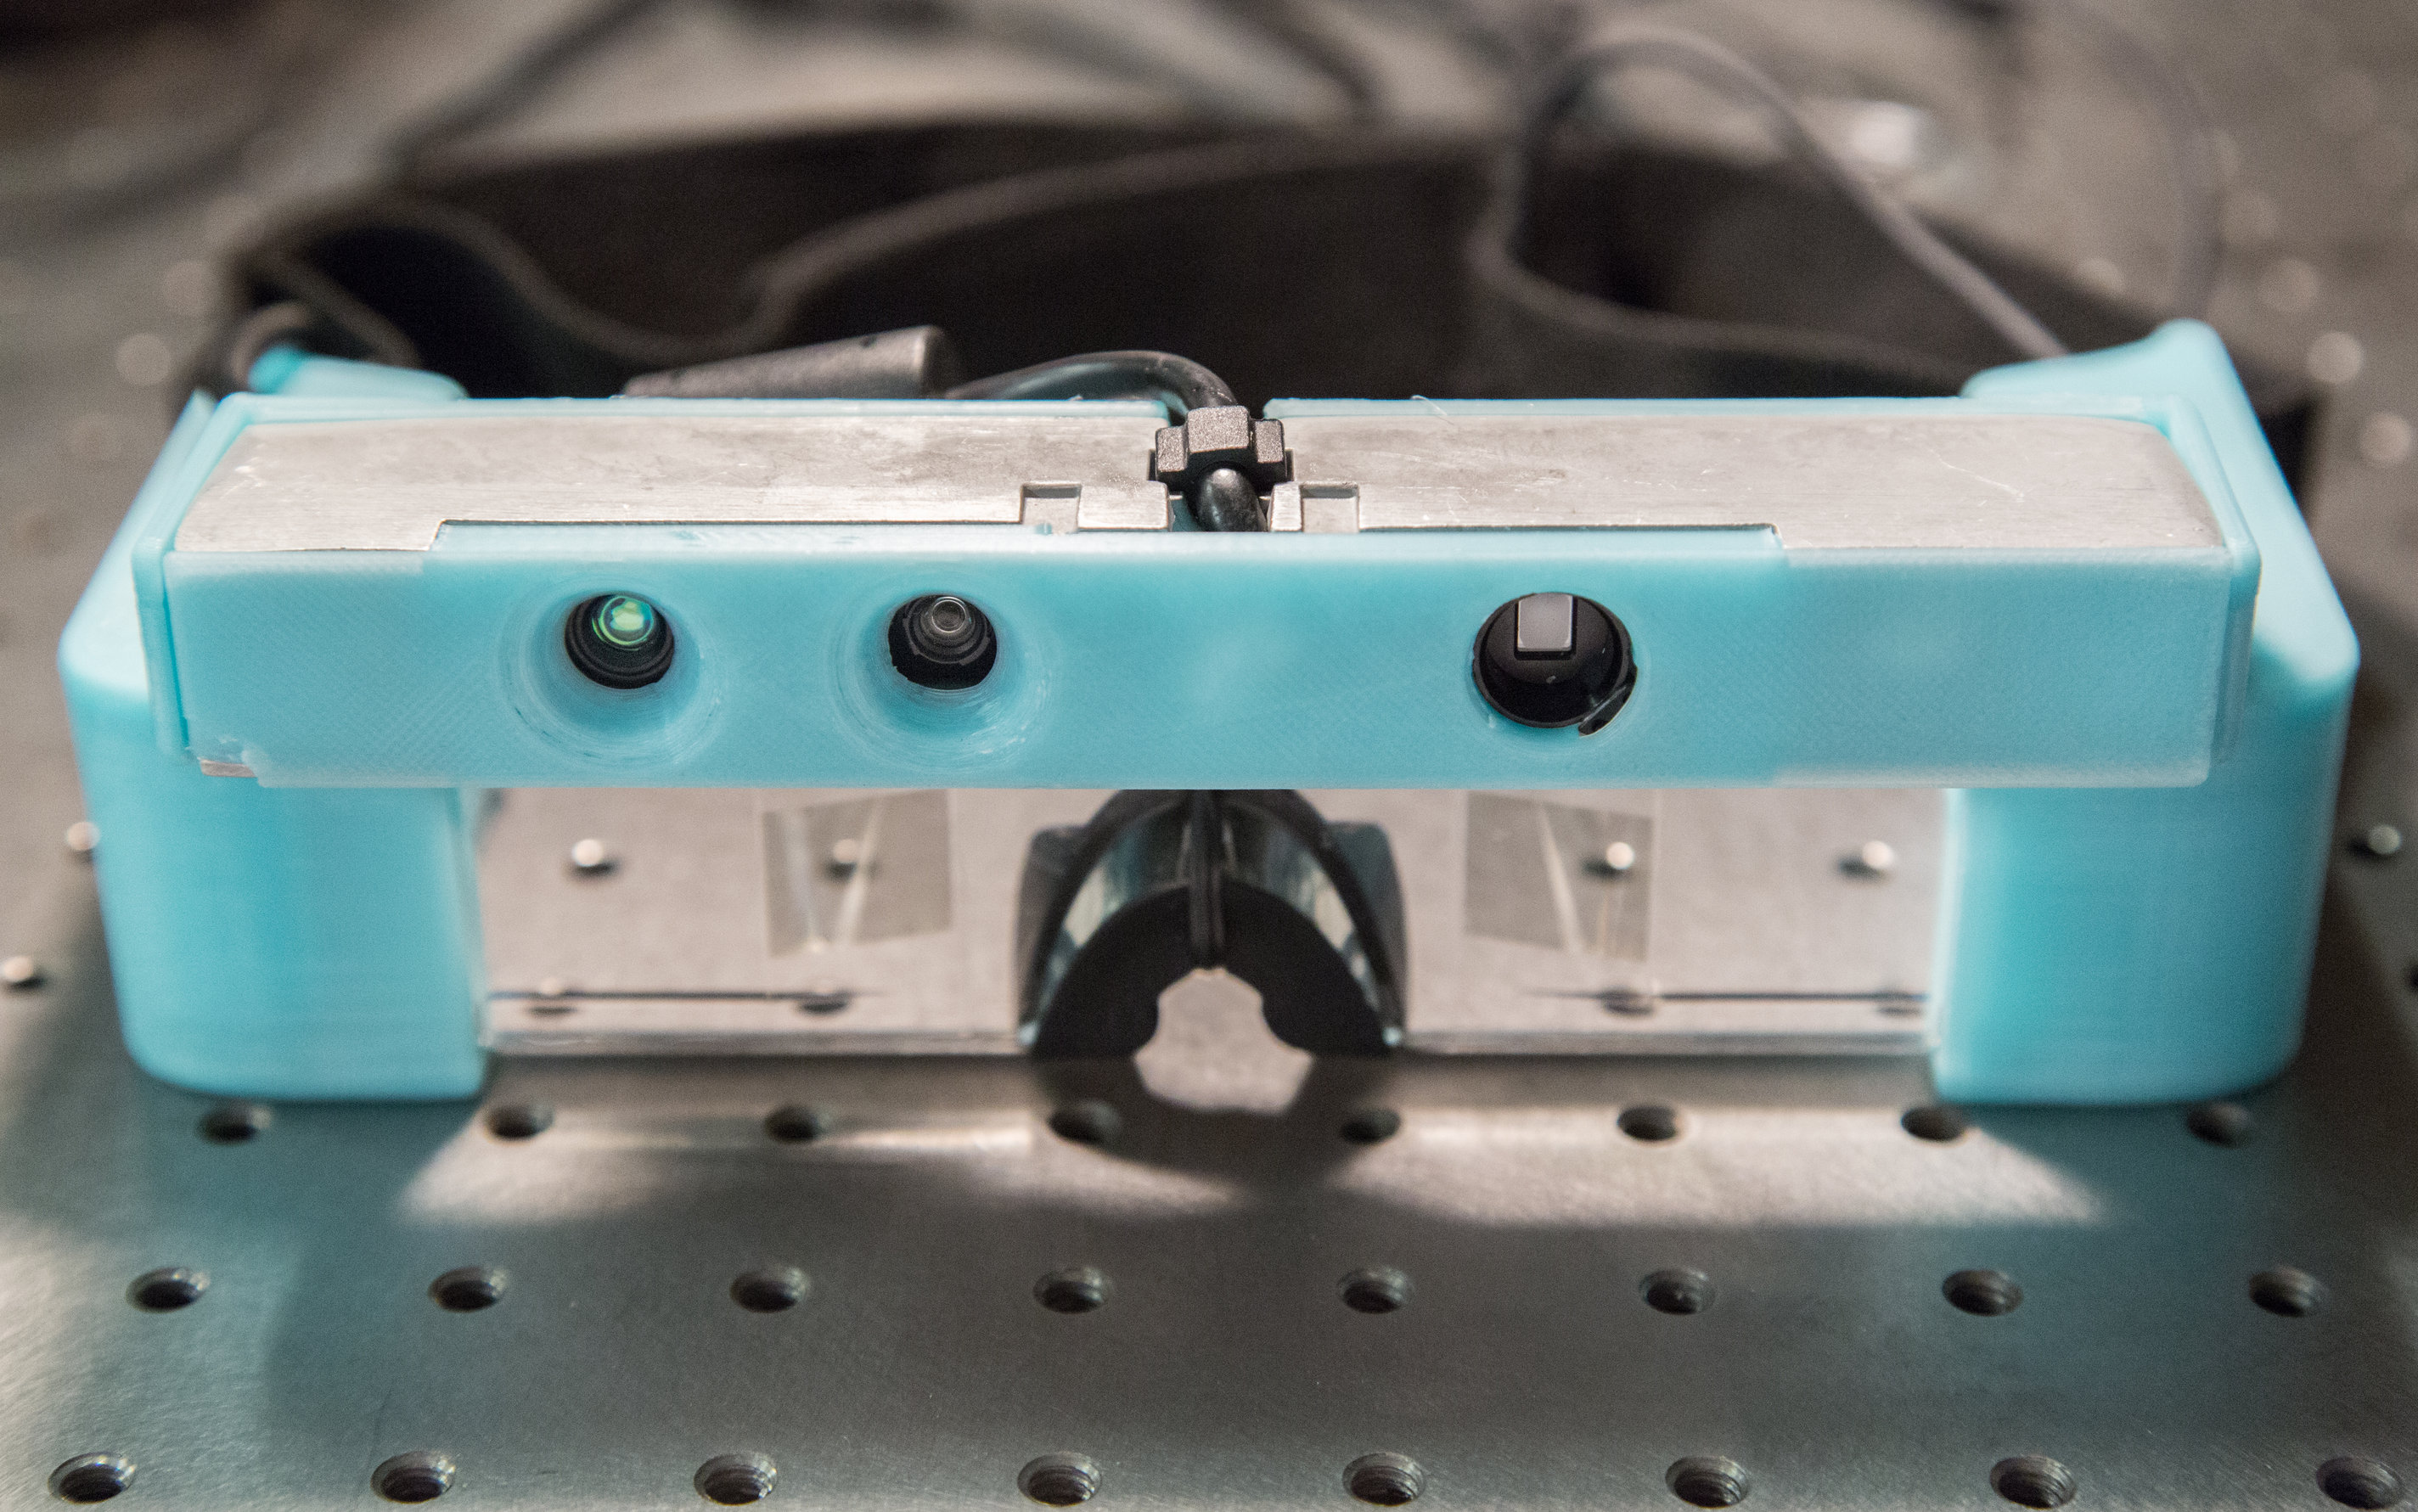
\includegraphics[height=1.2in]{ch4/diagrams/hdrglass/lowres/IMG_0263.jpg}
\caption{Front View}
\label{fig_second_case}
\end{subfigure}
~
\begin{subfigure}{.32\textwidth}
\centering
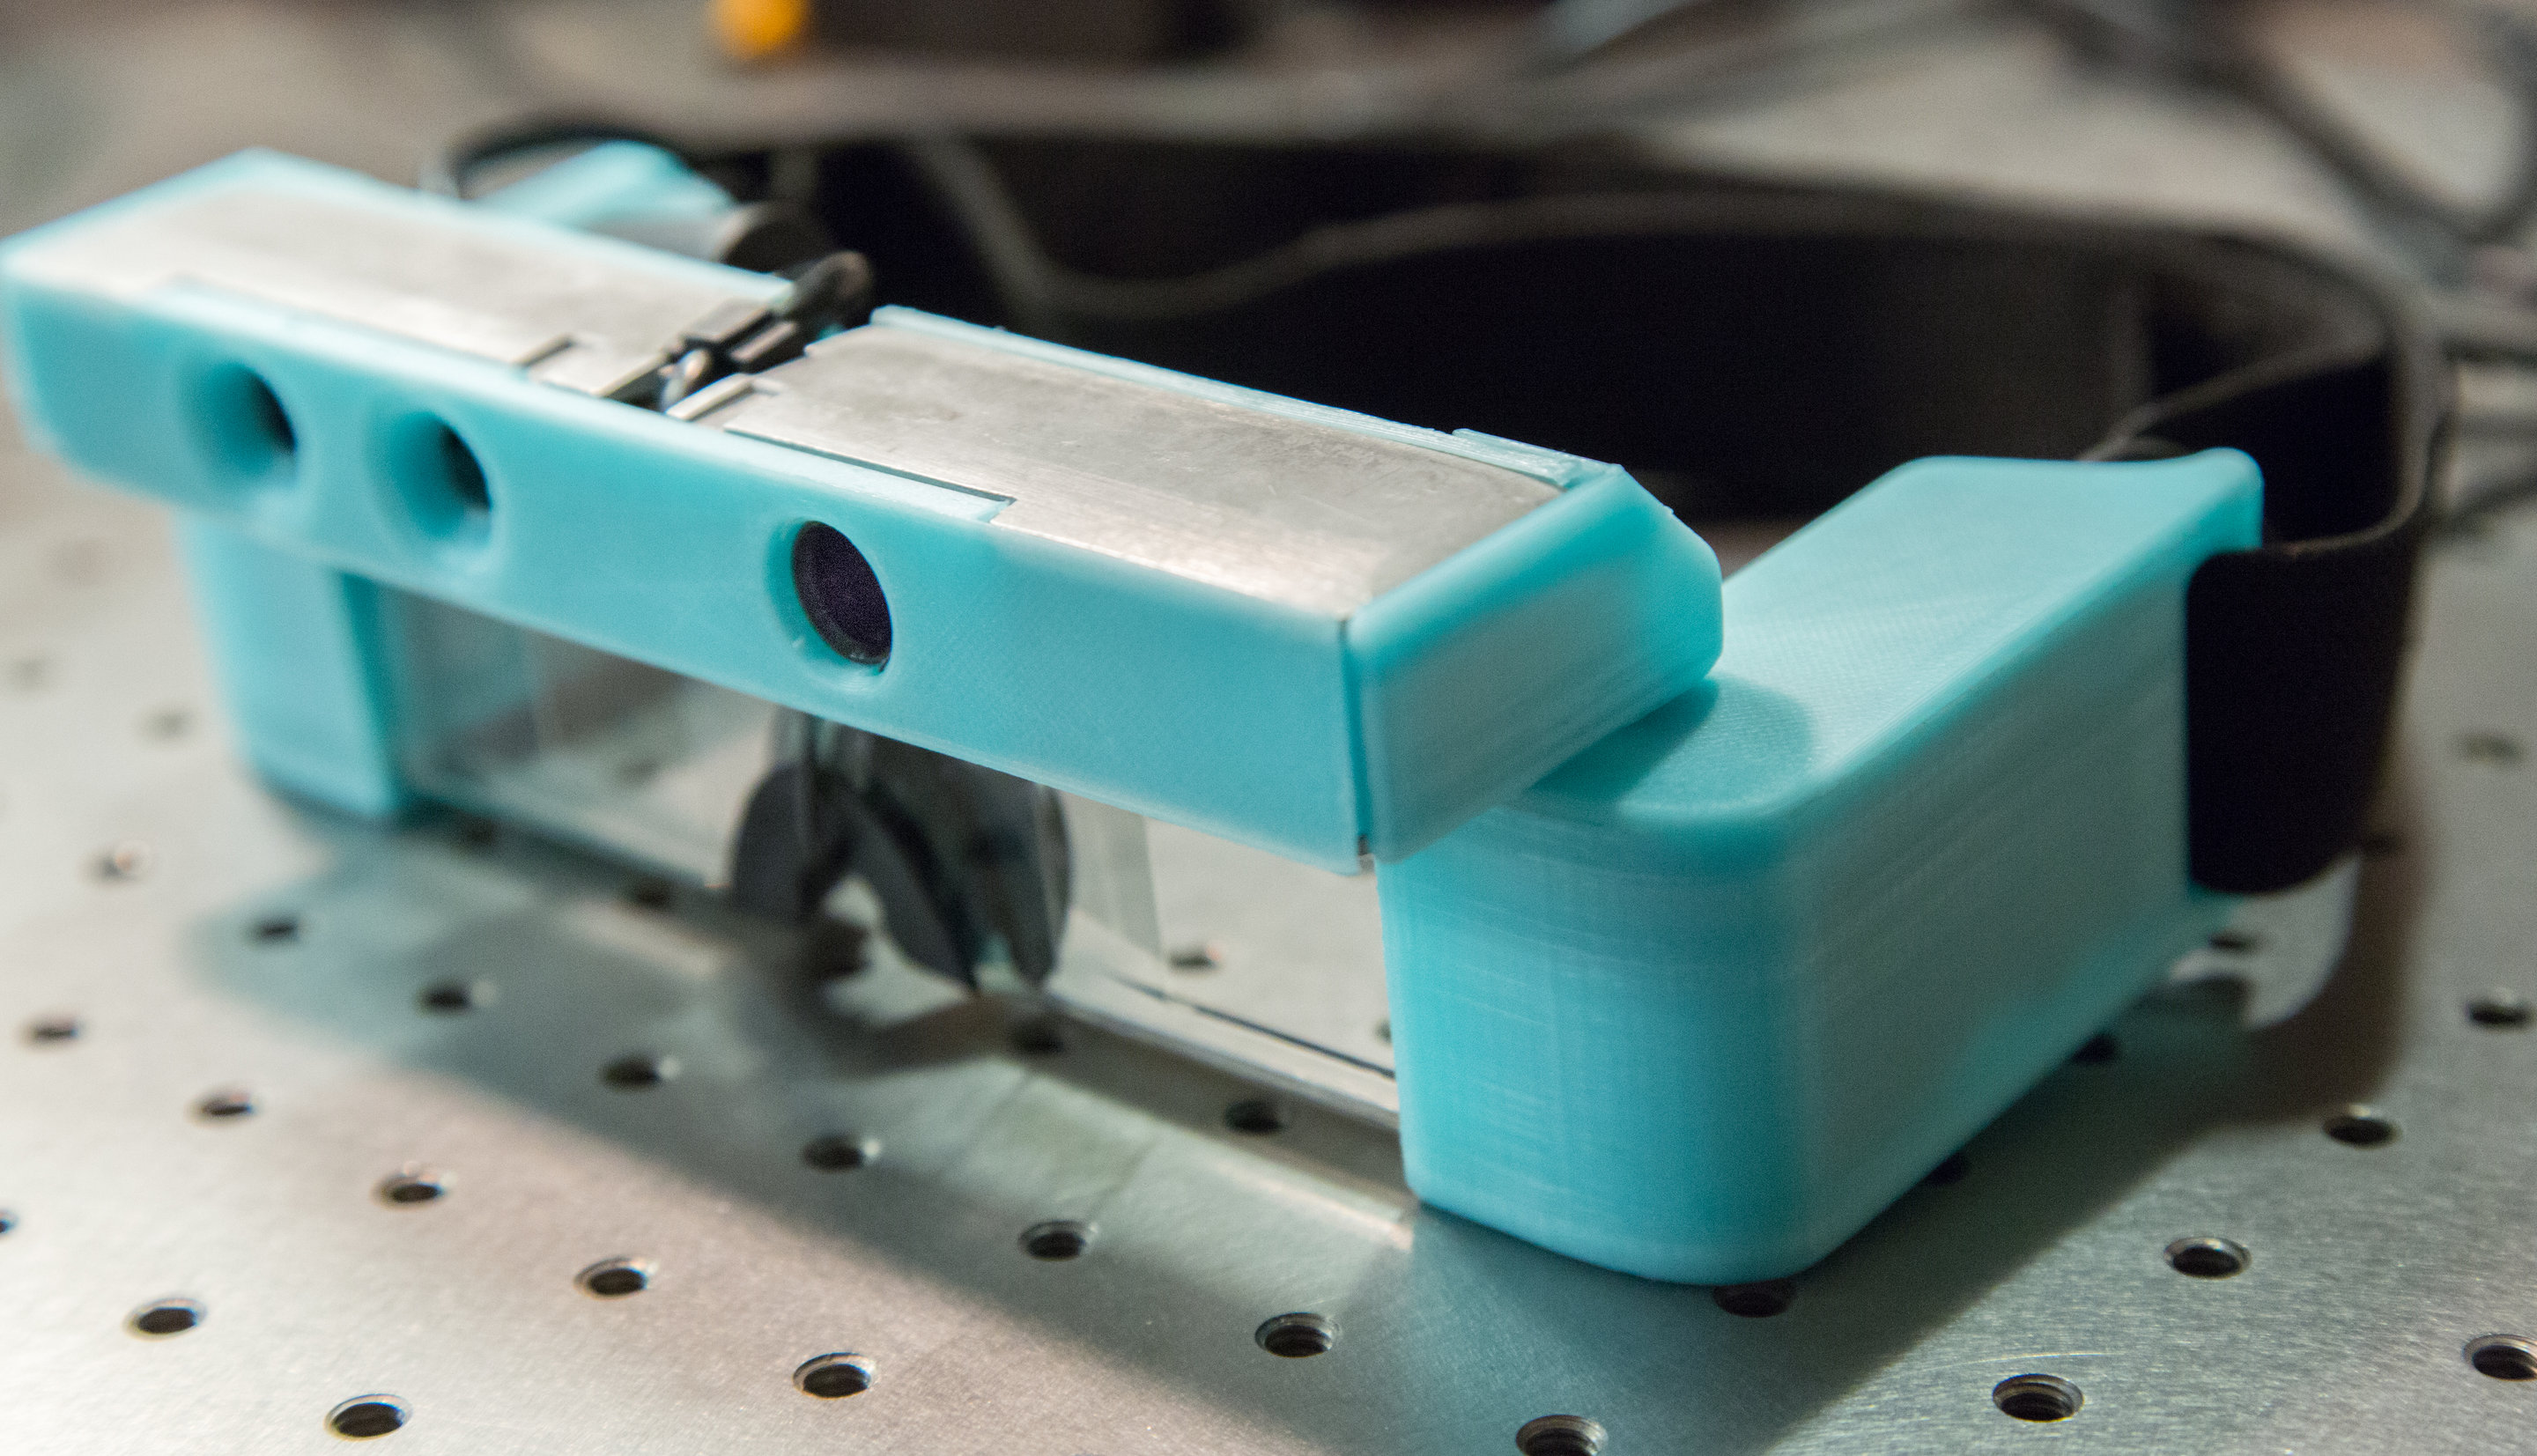
\includegraphics[height=1.2in]{ch4/diagrams/hdrglass/lowres/IMG_0258.jpg}
\caption{Side View}
\label{fig_first_case}
\end{subfigure}

\caption{Wearable Digital Eye Glass Prototype. The custom 3D printed design allows users to wear 
the digital glass in everyday life. The proposed algorithm can be utilized for improving the dynamic 
range of the camera and thus allowing the users to see ``better''. Notice that the proposed system 
not only allows users to see in high contrast scenes, it also enables night vision with the use of 
active depth sensors which project IR light patterns and reconstruct 3D information about the 
scene. This provides users the ability to see in extreme environment, and also allows for more 
robust tracking algorithms to be integrated with the eyeglasses.}
\label{fig_wearable_glass}
\end{figure*}


\subsection{Reversing the role of the user and camera: Sousveillance}
The use of the Kinect 3D sensing cameras in a different manner is proposed in this chapter, where 
the Kinect camera moves with the user so that it observes the real world in a similar fashion as the 
user observes it (or would have observed, in the case of a blind individual). Rather than having the 
Kinect camera watch the user, the user uses it to watch the environment. In one of the wearable 
implementations as shown in Fig.~\ref{fig_wearable_glass}, the Kinect camera is used to extract 
depth information from the environment being observed by the user.

There are numerous potential applications for such a system:
\begin{itemize}
\item Seeing and sensing aid \cite{mann2011blind}
\item EyeTap wearable Digital Eye Glass \cite{lo2012high, mann2012hdrchitecture, mann2012realtime}
\item 3D (sur/sou)veillance 
\item 3D scanning and reconstruction \cite{izadi2011kinectfusion}
\item Surface tracking and gesture input for wearable computers requiring both long and short range scanning
\end{itemize}

\subsection{The fundamental problem of sousveillance: Dynamic Range}
\begin{figure*}
\centering
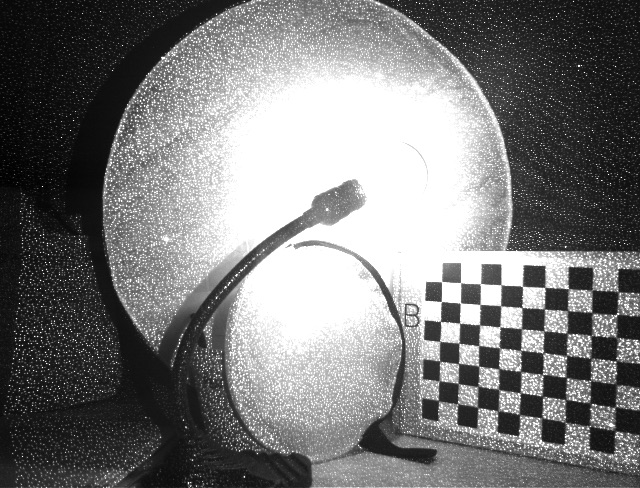
\includegraphics[width=3.0in]{ch4/diagrams/high_expo_light.jpg} 
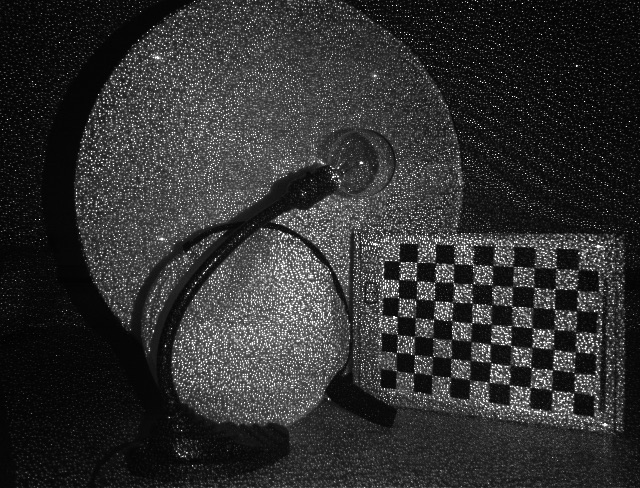
\includegraphics[width=3.0in]{ch4/diagrams/no_light_depth.jpg} \\
\caption{Fundamental dynamic range issues in depth-sensing cameras. The limited dynamic range 
of the sensor often creates blind spots in the scene. In this case, the light bulb blinded the sensor 
completely leaving a white patch on the scene even with an infrared camara. To overcome this, we 
can also deploy HDR approaches described in previous chapters.}
\label{fig:ir_range_issue}
\end{figure*}

Generally, surveillance is the monitoring of one's own property such as one's own living room, i.e., 
a space that one has control over. With surveillance, we can carefully place the camera in the 
optimal location. For example, in using the Kinect camera to observe a typical living room, the user 
will often give careful consideration to its placement, being sure to avoid placing it where sunlight 
might shine in from windows. The user may move lamps out of its field of view, in order to reduce 
glare that prevents it from working properly.  On the other hand, sousveillance involves seeing in a 
property that might not belong to the wearer, and the assumption of being static is often 
invalidated. For example, the gesture-sensing camera or seeing aid must function in any 
environment where we cannot demand the owner of the space to remove lamps that may be 
causing glare or similar problems.

When using the Kinect camera as a seeing aid, for self gesturing (gesture-sensing wearable 
applications), and marker or markerless surface tracking, it would be unreasonable to demand the 
environment to conform to the user's needs. For example, Fig.~\ref{fig:ir_range_issue} is a 
common scene where a light blub is presented in an indoor environment. When the light bulb is 
turned on, the sensor fails to pick up any information around the bright area due to the limited 
dynamic range of the sensor. 

Thus, the problem of dynamic range must be solved in the sousveillance device itself without 
requiring a  change in the environment. Fortunately, advances in sensor technology have enabled 
the miniaturization of sensors and their use in a robust camera array setup. One way to address 
the dynamic range limitation is to combine various sensor signals and create a superset which 
surpasses the capability of any individual sensor alone.

\subsection{Technology Behind the Microsoft Kinect system}
The Microsoft Kinect system employs the PrimeSense 3D sensing technology. The PrimeSense 3D 
sensor uses light coding to compute the scene volume, using active infrared (IR) 
illumination~\cite{shpunt2008depth,shpunt2010optical,shpunt2007depth}. The sensor then uses a 
CMOS image sensor to read the light coding infrared patterns back from the scene as shown in 
Fig.~\ref{fig:ir_range_issue}. The coded light is processed by the PrimeSense 
SoC~\cite{spektor2009integrated}, contained in the 3D sensor, to calculate depth information. In 
many cases, one may notice that the infrared sensors may fail to observe objects which have high 
reflectance property (glossy surfaces) or high absorbance property (matte black finish surfaces). In 
these difficult cases, the idea of HDR comes in as by carefully adjusting the exposures, the 
sensors can adapt and observe what was not possible to see otherwise.

\begin{figure*}
\centering
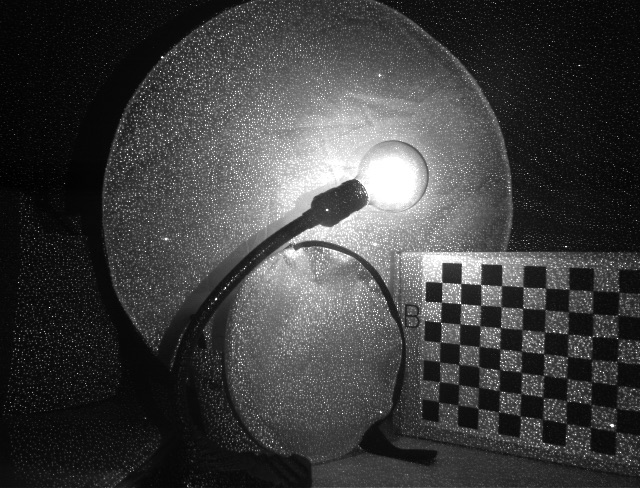
\includegraphics[width=3.0in]{ch4/diagrams/low_expo_light.jpg} 
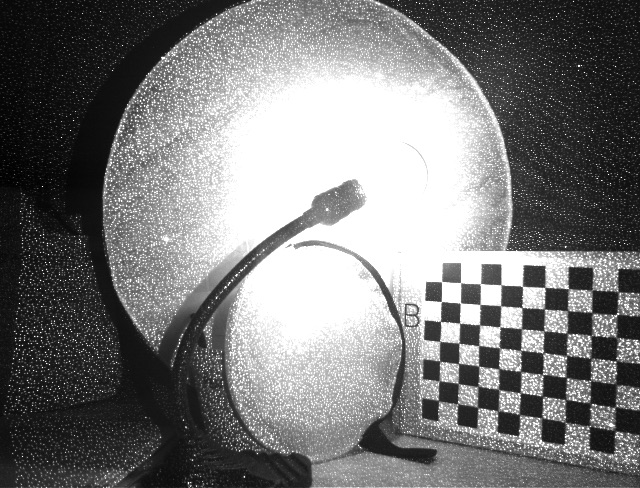
\includegraphics[width=3.0in]{ch4/diagrams/high_expo_light.jpg} \\
\caption{HDR image set with infrared-based depth sensing camera. By adding a ND-filter on top of 
the camera or alternating the exposure settings, two separate exposures of the same scene can be 
acquired. The important observation is that by combining both exposures, now we can obtain HDR 
image which improves not only in tonal range, but also the spatial range as the lower exposure 
now can see the over-exposed or close range, while the higher exposure image can now sense the 
far range.}
\label{fig:ir_hdr}
\end{figure*}

\section{Background and Theory}
In this section, we describe the geometric representation of the cameras and the formation of 
images with a pinhole camera model. These provide the fundamental principles for reconstructing 
images with the depth information from multiple Kinect cameras.  For consistency, the notation 
used in this chapter closely follows the conventions in~\cite{wei1994implicit,zhang2000flexible}. 
Then, we extend the discussion into High Dynamic Range (HDR) image composition with 3D data 
points. Here, we describe our novel algorithm that merges the differently exposed sets from the 3D 
data acquired with multiple Kinect cameras.

\subsection{Pinhole Camera Model and Perspective Projection}
To understand the geometric relationship between the camera and the scene, we first assume that 
the camera follows a pinhole camera model. That is, a scene view is formed by projecting a 3D 
point onto the image plane using a perspective transformation. 

Let's denote a 2D point on an image plane as $\mathbf{m}=[u, v, 1]^{T}$, and a 3D point in the 
scene as $\mathbf{M}=[X, Y, Z, 1]^{T}$, in homogeneous coordinates.

With a pinhole camera model, the relationship between 3D points $\mathbf{M}$ and its image 
projection $\mathbf{m}$ is given by\begin{equation}s \mathbf{m} = \mathbf{A} [ \mathbf{R} ~ 
\mathbf{t} ] \mathbf{M}, \label{pinhole_model}\end{equation}where the extrinsic parameters $
[\mathbf{R} ~ \mathbf{t}]$ describe the translation and rotation relationship between the real-world 
coordinate system and the camera coordinate system. 

The matrix $\mathbf{A}$ in Eq. \ref{pinhole_model} is called the intrinsic parameters of the camera, and is given by 
\begin{equation}
\mathbf{A} = 
\begin{bmatrix} 
  \alpha & \beta & u_{0}\\ 
  0 & \gamma & v_{0} \\
  0 & 0 & 1 \\  
\end{bmatrix}.
\label{intrinsic_parameters}
\end{equation} 
In Eq.~\ref{intrinsic_parameters}, ($u_{0}$, $v_{0}$) is the principle point, and $\alpha$, $\beta$, 
and $\gamma$ describe the scaling as well as the skew of the image in the $u$ and $v$ axes, 
respectively. In general, the camera may have a single focal length lens, and these intrinsic 
parameters only need to be estimated once per setup.
%$s[u v 1] = [fx 0 cx 0 fy cy 0 0 1][r11 r12 r13 r14 t1 ][X Y Z 1]$
\begin{figure}
\centering
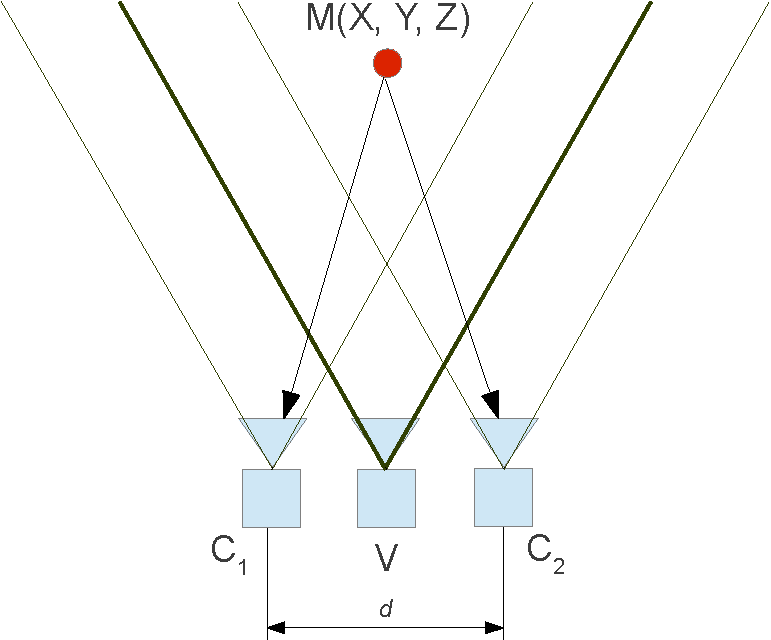
\includegraphics[width=2.5in]{ch4/diagrams/multi_virt_cam2.pdf} \\
%Camera Configuration and virtual cameras
\caption{This figure illustrates one of our proposed configuration. Each Kinect camera, $C_1$ and 
$C_2$, provides a 3D measure of the scene. With the 3D data, we can reconstruct the scene and 
re-position $C_1$ and $C_2$ onto a virtual camera $V$ at any arbitrary position. This configuration 
allows us to perform HDR composition as if the images were simultaneously captured from the 
same camera. The distance between the cameras $d$ can be estimated using a camera 
calibration method.}
\label{fig_v_camera}
\end{figure}
\subsection{Lens Distortion Correction}
Real lenses suffer from various level of distortions. For simplicity, we address the lens distortion problem by considering 
the radial and tangential distortion correction which can be modelled by a simplified Brown's 
model~\cite{brown1966decentering}
\begin{equation}
\begin{split}
%& x = (u - u_{0})\alpha,~y = (v-v_{0})\beta, \\ 
%& \bar{x} = x + \delta^{(x)}(x,y),~\bar{y}=y+\delta^{(y)}(x,y),\\
%& \delta^{(x)}(x,y) = x + x[k_{1} (x^2 + y^2) + k_{2} (x^2+y^2)^2], \\
%& \delta^{(y)}(x,y) = y + y[k_{1} (x^2 + y^2) + k_{2} (x^2+y^2)^2] \\
r &= \sqrt{(x^2+y^2)}, \\
x' &= x(1+k_1 r^2+k_2 r^4)+p_1(r^2+2x^2)+2p_2xy, \\
y' &= y(1+k_1 r^2+k_2 r^4)+p_2(r^2+2y^2)+2p_1xy
\label{eq_lens_distortion}
\end{split}
\end{equation}
where $(x', y')$ are the ideal pixel image coordinates after the distortion correction, $(x, y)$ are the 
real observed image coordinates centered at the principal point, and $k_{1}$, $k_{2}$, $p_1$, 
$p_2$ are the coefficients of the radial and tangential distortion, respectively.  These parameters 
can be estimated using a camera calibration method by providing a known geometry to the scene. 
One example would be to use a checkerboard pattern on a planar surface, and this technique will 
be discussed in the next section.

\subsection{Camera Calibration}
%Camera calibration is the preliminary step toward computer vision.
In order to combine the tonal and spatial information for our proposed setup, it is necessary to 
calibrate the cameras (i.e., estimate the extrinsic and intrinsic parameters described previously, 
and also estimate the camera response function for correcting the non-linearity in the HDR 
composition process.) Camera calibration is a well-studied problem in the computer vision field and 
numerous techniques have been proposed \cite{zhang2000flexible, mannist, 
robertson2003estimation} for correcting and estimating these parameters. Their implementations 
can be found in the common computer vision libraries such as the OpenCV camera calibration 
tools\footnote{Camera calibration with OpenCV:~\url{http://docs.opencv.org/2.4/doc/tutorials/calib3d/camera_calibration/camera_calibration.html}}.\begin{figure}
\centering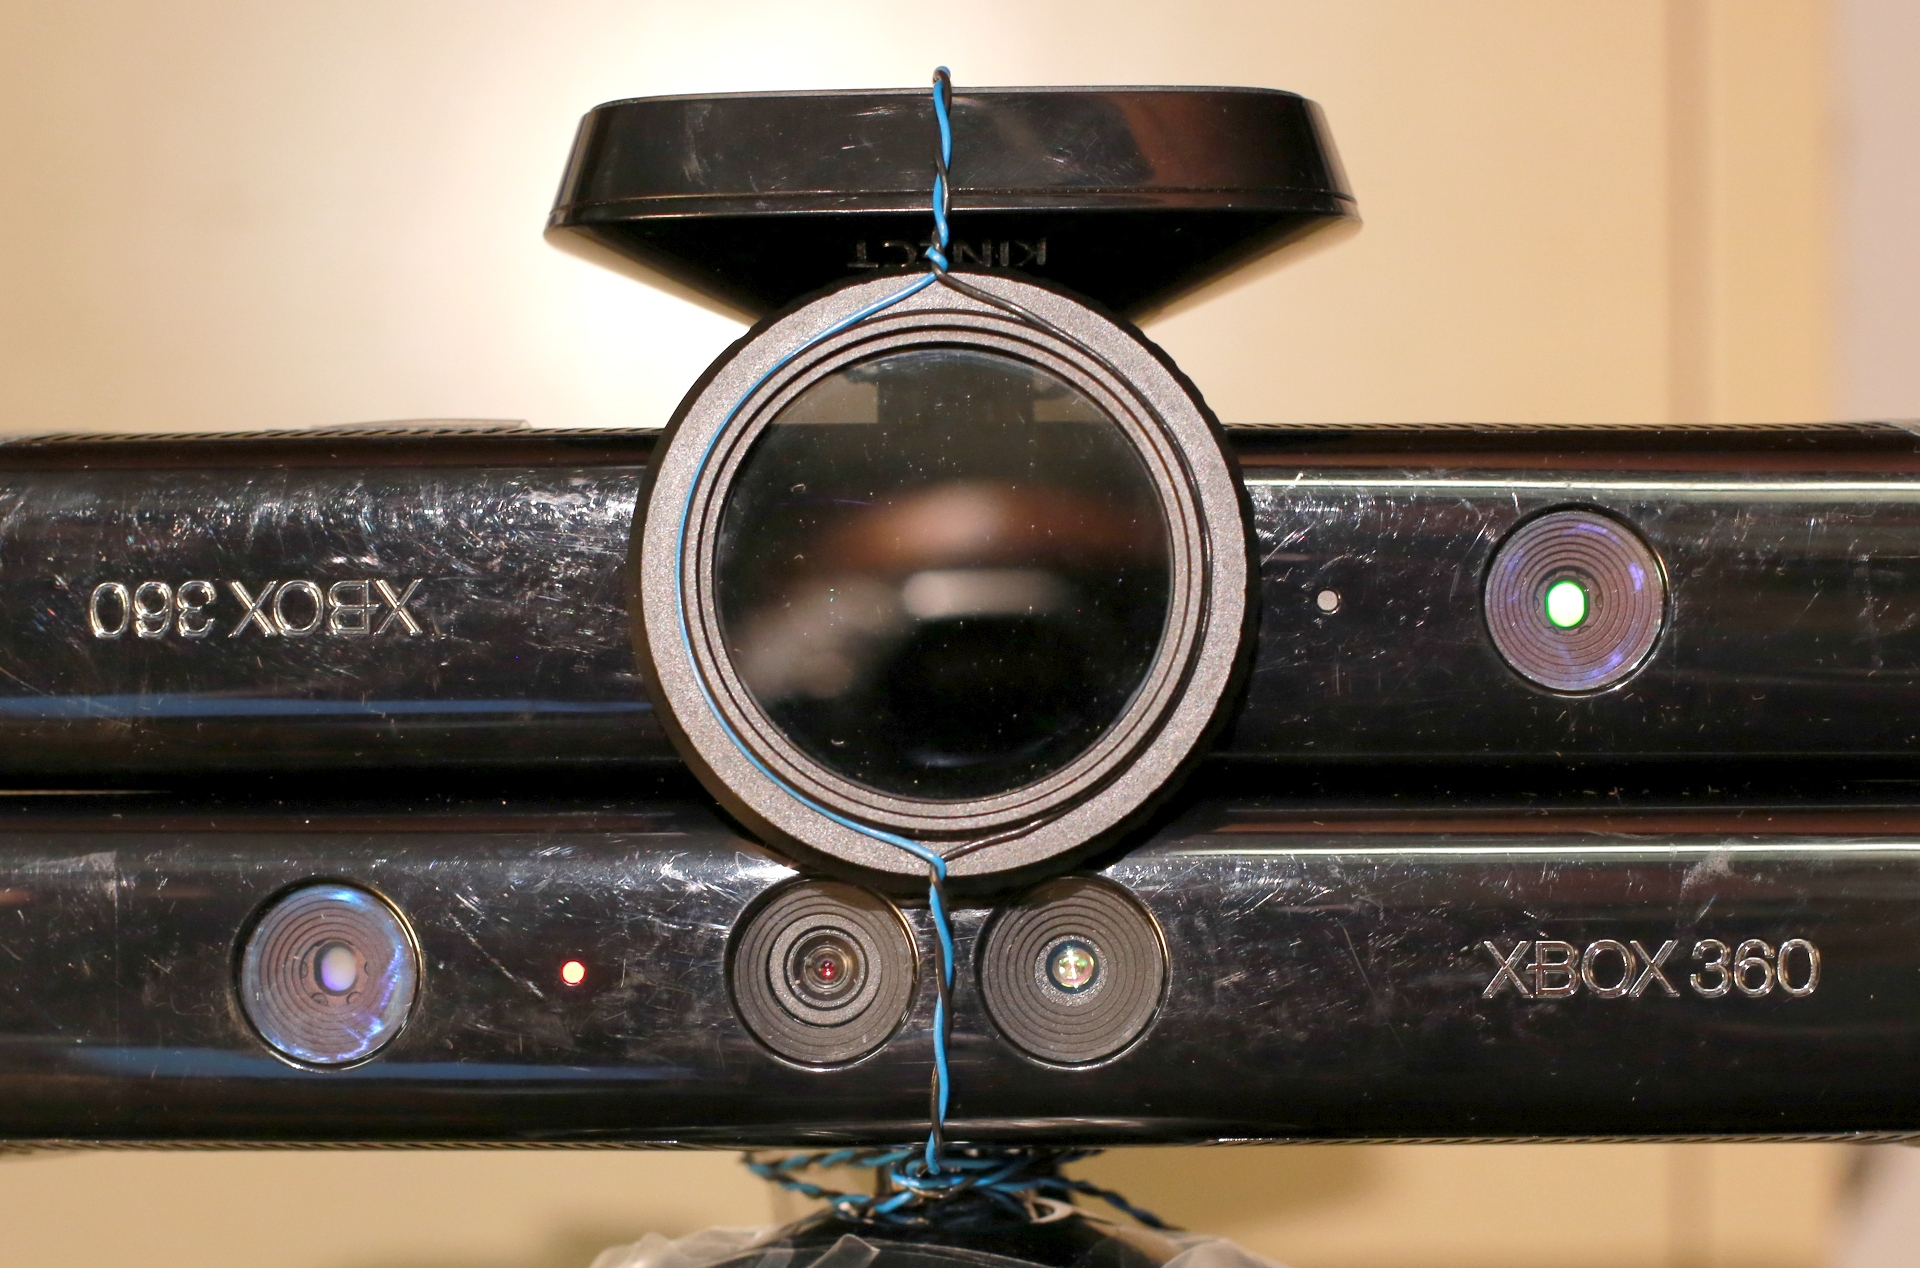
\includegraphics[width=3.4in]{ch4/diagrams/kinect_closeup} \\\caption{Our proposed 
configuration with two Kinect cameras. The upper Kinect camera is augmented with a polarized 
neutral density filter for manual adjustment of the exposure.}\label{fig_multiple_camera}\end{figure}


%XXX DESCRIBE THE CALIBRATION PROCESS XXX?
%Calibration techniques can be classified into one of the two categories: self-calibration and photogrammetric calibration. One key advantage of photogrammetric calibration technique is that 

\subsubsection{Geometric Calibration}For our configuration, we have the Kinect cameras 
positioned on top of each other as shown in Fig.~\ref{fig_v_camera}. It is possible to have these 
cameras further apart or closer together. However, the advantage of placing the camera closer 
together is that the cameras share a common field of view, which reduces the `holes' due to 
occlusion. Since the relative position of the cameras is fixed, in our setup, the calibration process is 
only required to be computed once -  increases the flexibility and portability of our 
approach.Equations (\ref{pinhole_model}) and (\ref{intrinsic_parameters}) provided a model for the 
camera relations. Given an image set of some known planar pattern (such as checkerboard), we 
can recover the intrinsic and extrinsic parameters of the cameras in (\ref{pinhole_model}) using the 
methods in \cite{zhang2000flexible}. Additionally, the lens distortion parameters described in 
(\ref{eq_lens_distortion}) are also modelled and thus estimated from the process.Once these 
parameters are estimated, the 3D data from each camera can be mapped to the real-world 
coordinates, allowing us to combine the data in the next step. 

%The initial step we first estimate the distortion parameters, intrinsic parameters of the individual cameras. This can be extracted easily by providing a xxx. 

In addition, we estimate the relative pose, $[\mathbf{R_{i}~ t_{i}}]$, for each $i$th Kinect in in the 
real-world coordinates to allow for a global registration of the 3D data. By setting one of the Kinect 
camera as a reference (origin), we can then describe the relative position of the Kinect cameras 
using simple matrices. All parameters extracted from our setup are summarized in 
Table~\ref{tab_calibration}.

\subsubsection{Photometric Calibration}Another key challenge in calibrating the Kinect is its lack of 
exposure controls. Instead of programming the camera for different exposure settings, in our 
configuration, a polarized variable neutral density filter was attached to one of the Kinect to reduce 
the exposure as shown in Fig.~\ref{fig_multiple_camera}. To capture differently exposed images on 
a Kinect, we programmed the Kinect for manual exposure, and thus the Kinect does not 
compensate for any changes to the lighting condition and alter the exposures unexpectedly.  Then, 
we manually adjust the filter to extract a set of images that varies in some known exposures for the 
recovery of the camera response function\cite{mannist}.

%\begin{figure}
%\centering
%\includegraphics[width=1.5in]{ch4/diagrams/bright.png} 
%\includegraphics[width=1.5in]{ch4/diagrams/dark.png} \\
%\includegraphics[width=1.5in]{ch4/diagrams/bright_depth.png} 
%\includegraphics[width=1.5in]{ch4/diagrams/dark_depth.png}
%%Camera Configuration and virtual cameras
%\caption{Multiple Exposures captured by the Kinects. The slight change in the camera position results in two images of the same scene rendered from different perspectives. The depth map is not affected by the darkening because the structured light code pattern is invariant to small changes in exposures. However, there is an increase in dynamic range in high contrast scene when the IR images were overexposed.}
%\label{fig_v_camera}
%\end{figure}

\begin{figure*}
\centering
\includegraphics[width=6.5in]{ch4/diagrams/hdr_3d_all.pdf} 
%\includegraphics[width=1.1in]{ch4/diagrams/kinect_ir_color_3/off_light_filter/depth.png} 
%\includegraphics[width=1.1in]{ch4/diagrams/kinect_ir_color_3/off_light_filter/ir.png} 
%\includegraphics[width=1.1in]{ch4/diagrams/kinect_ir_color_3/off_light_filter/rgb.png} \\
%(a) Tungsten light off with a variable ND filter attached \\
%\includegraphics[width=1.1in]{ch4/diagrams/kinect_ir_color_3/off_light/depth.png} 
%\includegraphics[width=1.1in]{ch4/diagrams/kinect_ir_color_3/off_light/ir.png} 
%\includegraphics[width=1.1in]{ch4/diagrams/kinect_ir_color_3/off_light/rgb.png}   \\
%% \vspace*{3pt}
%(b) Tungsten light off\\
%\includegraphics[width=1.1in]{ch4/diagrams/kinect_ir_color_3/on_light_filter/depth.png} 
%\includegraphics[width=1.1in]{ch4/diagrams/kinect_ir_color_3/on_light_filter/ir.png} 
%\includegraphics[width=1.1in]{ch4/diagrams/kinect_ir_color_3/on_light_filter/rgb.png} \\
%(c) Tungsten Light on with a variable ND filter attached \\
%\includegraphics[width=1.1in]{ch4/diagrams/kinect_ir_color_3/on_light/depth.png} 
%\includegraphics[width=1.1in]{ch4/diagrams/kinect_ir_color_3/on_light/ir.png} 
%\includegraphics[width=1.1in]{ch4/diagrams/kinect_ir_color_3/on_light/rgb.png}  \\
%(d) Tungsten light on\\
%Camera Configuration and virtual cameras
\caption{Notice that the depth map is not significantly affected by the darkening filter. The 
structured light code pattern is invariant to small exposure differences; however, there is an 
increase in dynamic range in high contrast scene when the IR images were overexposed by the 
tungsten light. The depth composition algorithm is described in Section~\ref{sec_hdr_depth_map}.}

\label{fig_all_camera}
\end{figure*}
\begin{figure*}
\centering
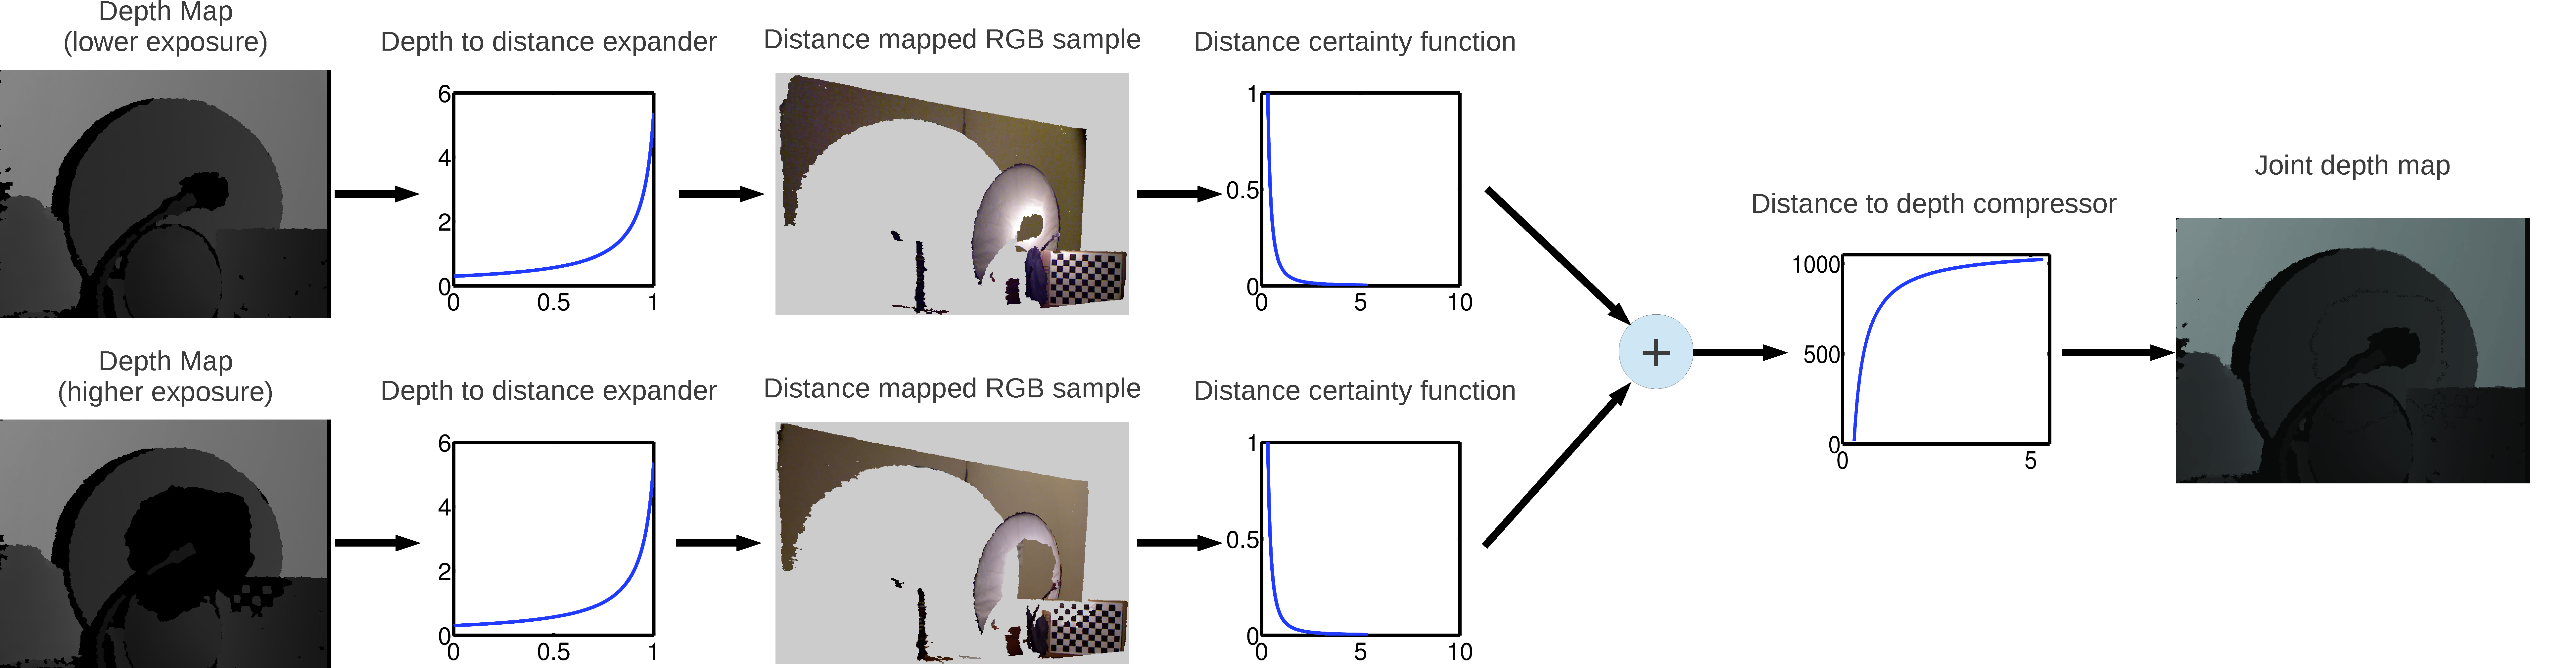
\includegraphics[width=7in]{ch4/diagrams/jason_hdr.pdf} 
\label{fig_jason_dep_hdr}
\caption{Depth map composition using our proposed algorithm. We combine two different depth 
maps by performing a weighted sum over the certainty function described in 
Eq.~\ref{eq_depth_sum}. There is a slight contour in the area were the depth map is undefined as 
shown in the right most image. These can be addressed by applying spatial filters on the depth 
map based on the geometry.}
\end{figure*}
\subsubsection{Summary}
%\begin{figure}
%\end{figure}


%describe the algorithm behind the registration and calibrations behind the camera
%show the rgb images
%alignment algorithm(s): using checker board
%and it is a real-time process? because once it is calibrated, our setup wont' require any other calibrations
\begin{table}[h]\footnotesize
\centering
  \caption{Parameters estimated from the camera calibration process}
  \label{tab_calibration}
    \begin{tabular}{|p{2.0cm}|l|p{4.0cm}|}
        \hline
       \bf{Parameter(s)}        &  \bf{Type}      &  \bf{Description}                                                        \\ \hline
        $\mathbf{A}_{ci}$, $\mathbf{A}_{ri}$  & Intrinsic & Focal length, principle points, and skews for the color camera and the infrared camera of the $i$th Kinect \\ \hline
        $kc_{1i}$, $kc_{2i}$, $pc_{1i}$, $pc_{2i}$  & Intrinsic & Lens distortion coefficients for the color camera of the $i$th Kinect \\  \hline
        $kr_{1i}$, $kr_{2i}$, $pr_{1i}$, $pr_{2i}$  & Intrinsic & Lens distortion coefficients for the infrared camera of the $i$th Kinect \\ \hline
        $\mathbf{R}_i$, $\mathbf{t}_i$             & Extrinsic & Geometric relations between the infrared camera and the color camera of the $i$th Kinect \\ \hline
        $\mathbf{R}_{ij}$, $\mathbf{t}_{ij}$    & Extrinsic & Geometric relations between the $i$th and the $j$th Kinect in the scene \\
        \hline
        $f_r(q)$, $f_g(q)$, $f_b(q)$    & Photometric & The camera response function for each color channel\\
        \hline
    \end{tabular}
\end{table}

%table that summarize what's going to be extracted from the calibration process
Table~\ref{tab_calibration} summarized the parameters required for the 3DHDR reconstruction step. For our experiment, we have used two Kinect cameras and the first Kinect is set as the reference camera. For example, the matrices $\mathbf{R}_{21}$ and $\mathbf{t}_{21}$ defines the transformation of how 3D data is transformed from the second Kinect camera to the first Kinect camera. Lastly, the photometric calibration  provided us a camera response function that describe the non-linear relationship in both the IR and the color camera.

\subsection{3D Point Cloud Reconstruction from Kinect Cameras}
Each of the Kinect camera provides a 3D measure of the scene with the color camera and the infrared-based depth camera as shown in Fig~\ref{fig_multiple_camera}. The IR camera receives the structured light pattern emitted by the IR laser projector for depth reconstruction. The depth measure $[x_d, y_d, z]^T$ corresponds to a point $[X_i,Y_i,Z_i]^T$ in the real-world coordinates, and the conversion from image coordinate (in pixel) to real-world coordinates (in meter) can be computed with the following equations
\begin{equation}
\begin{split}
X_i &= (x_d - p_x) * z / f_d,\\
Y_i &= (y_d - p_y) * z / f_d, \\
Z_i &= z, \forall \{ z_{min}<z<z_{max}\}
\label{3D_kinect_color}
\end{split}
\end{equation}
where ($x_d$, $y_d$) is the image/pixel coordinate of the depth map image, $z$ is the depth measurement in meter, ($p_x$, $p_y$) is the principle point, $f_d$ is the focal length of the depth camera, and $i$ is the index for the $i$th point in space. In case z is out of the range of $z_{min}$ or $z_{max}$, we simply ignore these values in the computation.

Since the position of the IR and color cameras are fixed, we can relate the depth information to the color image by performing a transformation using the intrinsic and extrinsic parameters estimated previously. To extract the RGB component for each point $\mathbf{M_i} = [X_i, Y_i, Z_i, 1]^T$, $i=1,..,m$ where m is the number of valid depth readings from the Kinects, we project $\mathbf{M_i}$ onto the the camera coordinates of the color camera using the intrinsic and extrinsic parameters estimated earlier to obtain the pixel coordinates in the RGB image, and then we aggregate these values to create our point cloud data point $\mathbf{\tilde{M}_{i}}$ along with its exposure $k_i$ 
\begin{equation}
\begin{split}
[u_i'~v_i'~1]^T &=  \mathbf{A}_{ci}[\mathbf{R}_i~\mathbf{t}_i]\mathbf{M}_i \\
[r_i, g_i, b_i, k_i]^T &= \mathbf{I}(u_i', v_i')
\label{eq_3D_rgb_lookup}
\end{split}
\end{equation}
where $\mathbf{R}_i$ and $\mathbf{t}_i$ defines the rotation and translation of the camera position from the IR camera to the color camera coordinates. Since the projection may result in a non-integer pixel coordinate for $(u_i', v_i')$, we would estimate its value by performing a linear interpolation on the neighboring pixels in the color image $\mathbf{I}$. From each Kinect, we construct a set of point cloud data $\mathbf{\tilde{M}_{i}} = [X_i, Y_i, Z_i, r_i, g_i, b_i, k_i]^T$ which consists of a 7-dimensional vector of the spatial and tonal information about the scene.


%\section{3D High Dynamic Range Imaging with a single Kinect} 
%\section{3D High Dynamic Range Imaging with a single Kinect} 
\section{High Dynamic Range Depth Map}
\label{sec_hdr_depth_map}
The Kinect camera contains the source of the projected IR pattern as well as the IR image sensor. Based on the observation of the distortion in the pattern of the scene, the device is able to compute the distance of the objects in the view. The observation, however, is affected by the material property and the distance of the objects. The objects are usually overexposed in close proximity to the camera and the pattern reflected off the objects at far are too dark and underexposed. This becomes a problem for the camera to determine the distance of the objects that are not well exposed. Due to the limited dynamic range per exposure setting, the perceived patterns by the infrared camera are lost in the over- or under-exposed areas of the scene.

The dynamic range problem can be resolved by capturing multiple exposures of the scene using the infrared camera. At the lower exposure, the details of closer objects is more visible to the IR sensor, while at the higher exposure, the details of far objects become more visible. For depth maps recovered from differently exposed IR images, the unknown depths, due to the lost details from one exposure, could be compensated by another. The collection of depth maps forms a high dynamic range depth map, which allows a greater coverage of depth calculation under a more diverse lighting condition.
\subsection{Comparagram Of Depth Map}

A comparagram is a cross histogram of two images of different exposures \cite{mannwyckofftr}. A comparagram reveals the comparametric relationship of the outputs of the same camera with different exposure settings. In our purpose of extending the depth map range based on the Wyckoff set of depth maps, we attempt to directly observe the relationship between the depth maps produced by the infrared images from different exposure settings. The resulting comparagram in Fig.~\ref{fig_various} shows that the known depth values from the images of the Wyckoff set are the same. Therefore, the response $f(*)$ of the depth value $d$ is simply $f(d) = d$.
\subsection{Compositing Of Depth Map}
The resulting comparagram in Fig.~\ref{fig_depth_parts} and Fig.~\ref{fig_all_camera} showed that the depth values are invariant to slight changes to exposures on the infrared sensor. In case of a scene with IR light source, a darkening filter can improve the depth map reconstruction because it reduces the exposures (see Fig~\ref{fig_all_camera}) in the over-saturated area. To combine the depth maps for the HDR reconstruction with a single Kinect, we adapt to the composition method described by \cite{mannwyckofftr} and apply certainty (or weight) on the estimated distance value of different depth maps. In contrast to \cite{mannwyckofftr}, the certainty function for the distance value is not based on the camera response of the infrared sensor. Instead we design the certainty function based on the sensitivity of the depth map to distance conversion. Denote $g(r)$ as the distance response function that converts the known distance $r$ of the objects in meters to depth values and $g^{-1}(d)$ as its inverse response, we obtain the certainty function by taking the derivative of $g(r)$ with respect to distance. According to \cite{mann2011blind}, we could convert the disparity map to depth map using the following equation
\begin{equation}
r = g^{-1}(d) = 1/(\alpha \cdot d + \beta)
\end{equation} 
where $\alpha$=$-0.0030711016$ and $\beta$=$3.3309495161$ are the parameters extracted from the least squared regression. Its certainty function \begin{equation}
c(r) = \frac{\delta g(r)}{\delta r} = 
\begin{cases} \frac{-1}{\alpha \cdot r^2}, 
			& \mbox{if } r_{min} \le r \le r_{max} \\
			0, & \mbox{otherwise}
 \end{cases}
\end{equation}
where $r_{min}$$\approx$$0.3$m and $r_{max}$$\approx$$5.3$m are calibrated based on our Kinect cameras.
Lastly, the joint estimate of distance from two sensors with different exposure settings is expressed as the weighted sum per pixel
\begin{equation}
r_{joint} = \frac{\sum c(r_i) \cdot r_i}{\sum c(r_i)}
\label{eq_depth_sum}
\end{equation}
where $r_i$ denotes the estimated distance value observed by the $ith$ sensor.
\begin{figure*}
\centering 
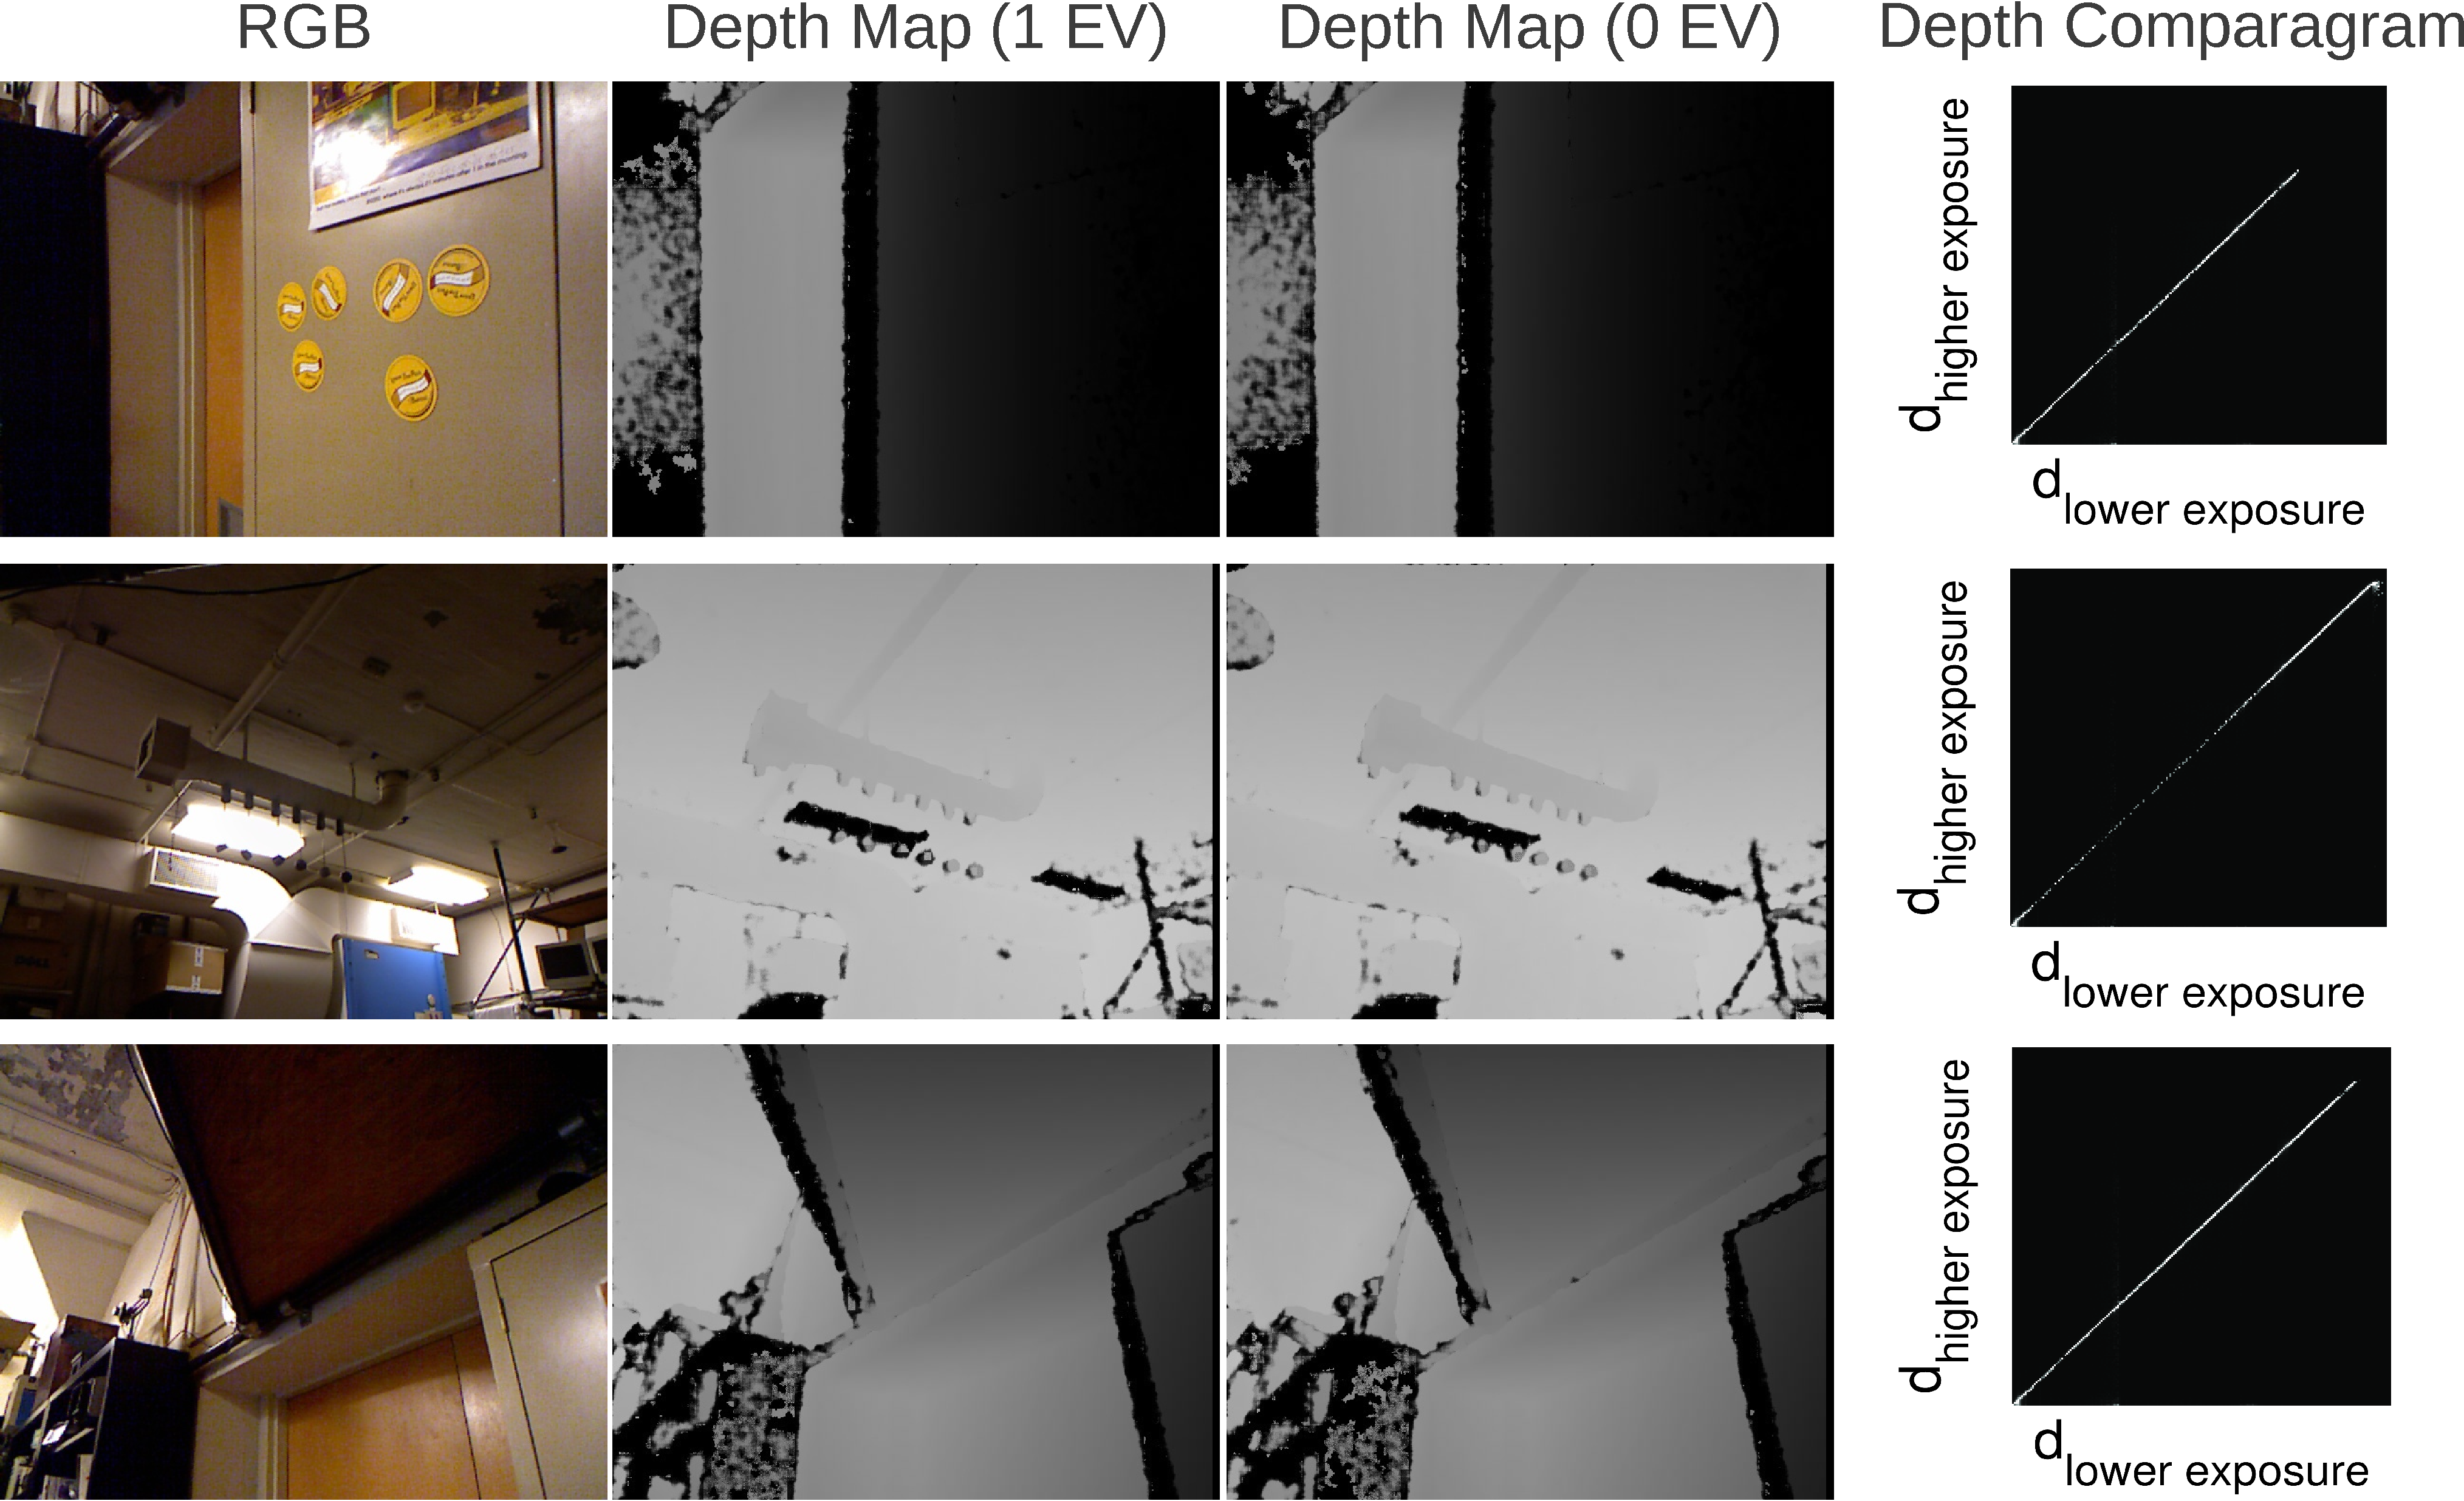
\includegraphics[width=6.5in]{ch4/diagrams/jason_depth.pdf} 
\caption{Image pairs used for comparagram construction. Three different Wyckoff sets of two depth maps were captured to cover the full range of depth values. The exposure difference between the bright and the dark infrared image is 1 EV apart. The resulting depth map comparagram per Wyckoff set is shown in the right most column of the figure. Each covers a partial range of depth values in its comparagram.} 
\label{fig_depth_parts} 
\end{figure*}
%\begin{figure} 
%\centering 
%\includegraphics[width=0.5\columnwidth]{ch4/diagrams/jason_comparagram.pdf} 
%\caption{The aggregated comparagram using all comparagrams constructed of partial depth range in Fig.
%\ref{fig_depth_parts}.}
%\label{fig_aggregated} 
%\end{figure}
\begin{figure*} 
\centering 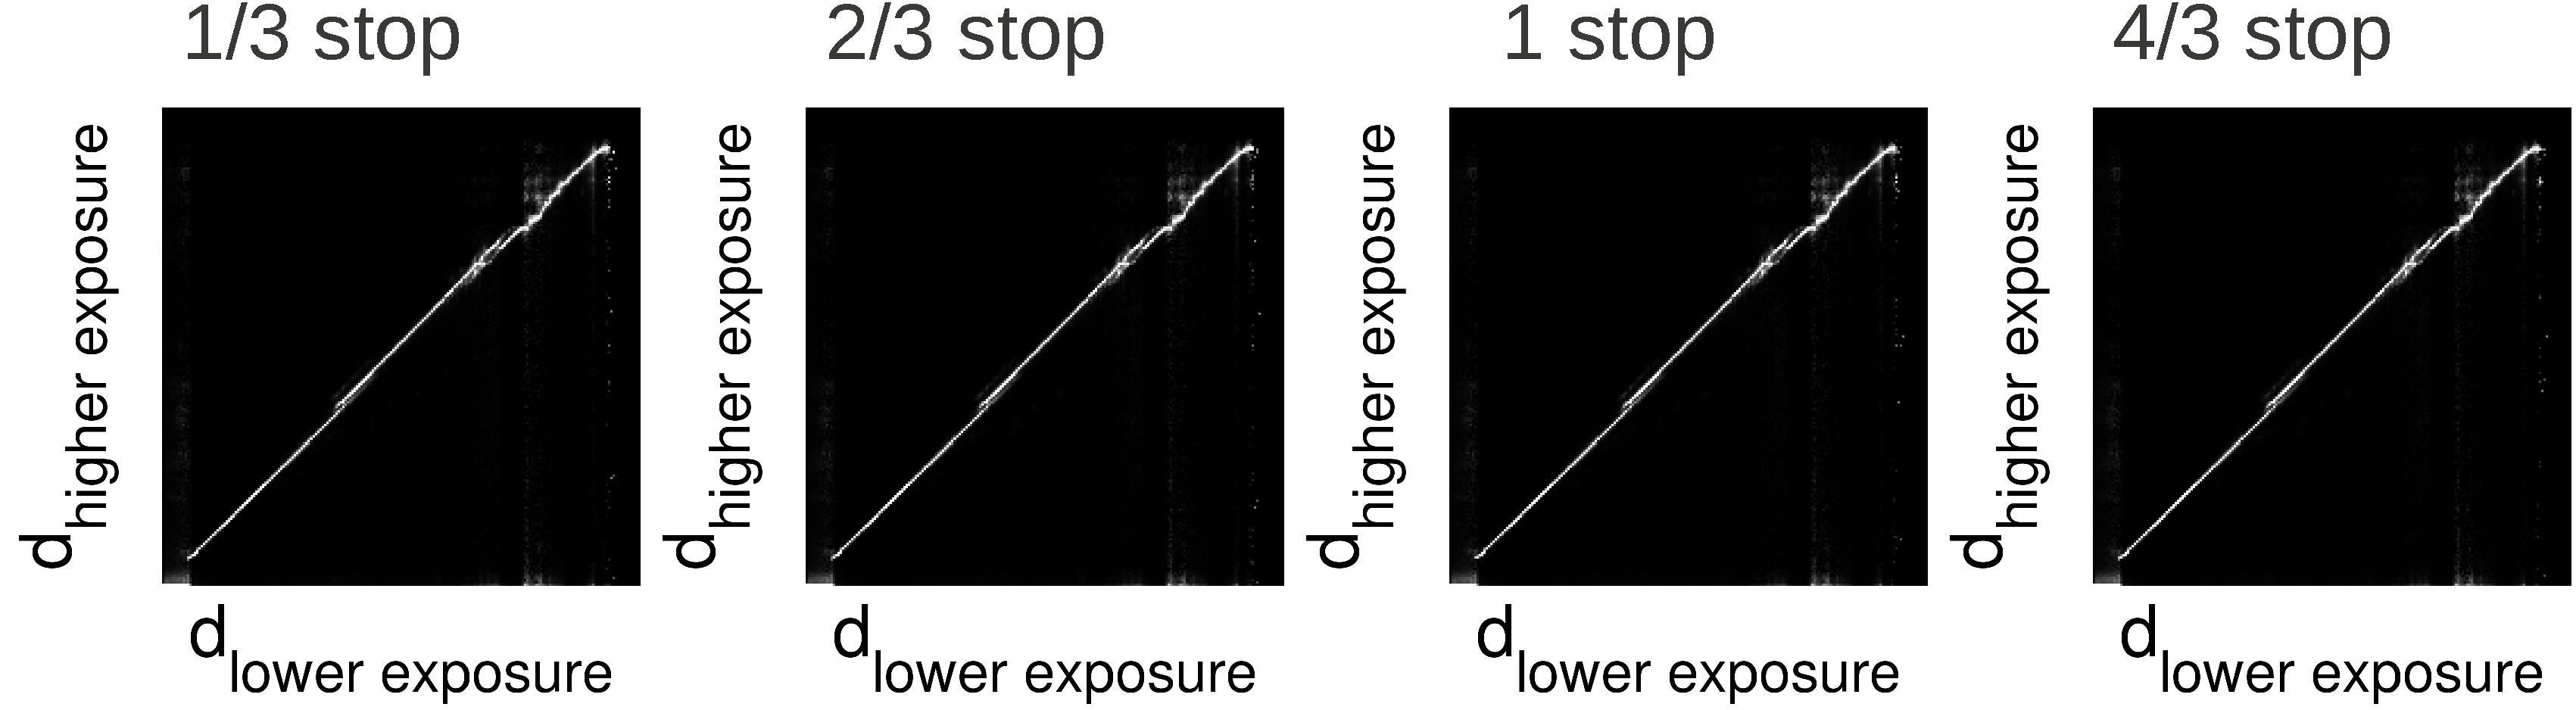
\includegraphics[width=6.5in]{ch4/diagrams/jason_collection.pdf} 
\caption{Comparagram of depth maps taken at various exposure differences. The comparagrams exhibit the same linear mapping of depth value obtained from infrared image pairs that are 1/3, 2/3, 1 or 4/3 stop apart.}
\label{fig_various} 
\end{figure*}


\section{3D High Dynamic Range Composition with Kinect(s)} 
High Dynamic Range imaging has been discussed extensively in the literature. By combining differently exposed images of the same subject matter, we can further extend the dynamic range of the sensors. In Fig.~\ref{fig_all_camera}, we see that it is possible to capture a higher dynamic range with the Kinect by taking multiple exposures of the same subject matter with a Kinect that is augmented with a polarized variable ND filter. In this section, we will discuss our novel technique for combining the data for producing an HDR 3D point cloud that has higher dynamic range in both tonal and spatial range that cannot be possibly captured by a single exposure. For simplicity, we will first discuss the approach with a single Kinect for capturing a static scene. The images are captured by adjusting the exposure on the variable ND filter and we assume that the camera and the scene are both static. Then, we propose an approach for constructing 3DHDR from data captured simultaneously from multiple Kinect cameras. One key contribution of this chapter is the novel approach and the unique configuration that allows simultaneous capturing, reconstruction, and rendering of 3DHDR data stream from 3D range sensing cameras. 

\subsection{Backgrounds}
In our configuration, we capture a set of images, possibly synchronously among the Kinects, to produce two point cloud data sets that capture differently exposed images of the scene along with their 3D data: $\mathbf{\tilde{M}_{i}}$ and $\mathbf{\tilde{N}_{j}}$, $i=1,..,m$, $j=1,..,n$, where m and n are the number of point clouds data reconstructed from Kinects.

We denote $f$ and $f^{-1}$ as the `camera response' and the `inverse camera response' respectively. A pixel, $p$, is the camera response of quantigraphic measure, $q$, at a selected exposure level, $k$, which can be expressed as $p = f(kq)$. Inversely, the estimate of $q$ from a single exposure is $\hat{q} = f^{-1}(p)k_i^{-1}$. Thus the joint estimate $\hat{q}_{joint} = f_{joint}(k_1\hat{q_1}, .., k_i\hat{q_i}, .., k_n\hat{q_n})$ can be computed using the methods proposed by \cite{mannist,robertson2003estimation,ali2012ICASSP} based on a Wyckoff set \cite{wyckoff1962experimental} of size $N$, for $N \ge 1$.

\subsection{HDR Composition with a Single Kinect}
\label{sec_single_kinect}
Similar to the approach proposed in \cite{lo2012high}, we can easily combine the differently exposed images using the weighted sum approach. The HDR image undergoes a real-time tonemapping algorithm described in previous chapter~\cite{lo2012high} to allow for displaying on low dynamic range (LDR) displays. Additionally, the depth map composition will create a depth map that has fewer missing depth points than any of the single depth maps. Using Equation (\ref{3D_kinect_color}) and (\ref{eq_3D_rgb_lookup}), we can then create a 3D point cloud data as our desired HDR output. 

\subsection{Simultaneous HDR Composition with Multiple Kinects}
\begin{figure}
\centering
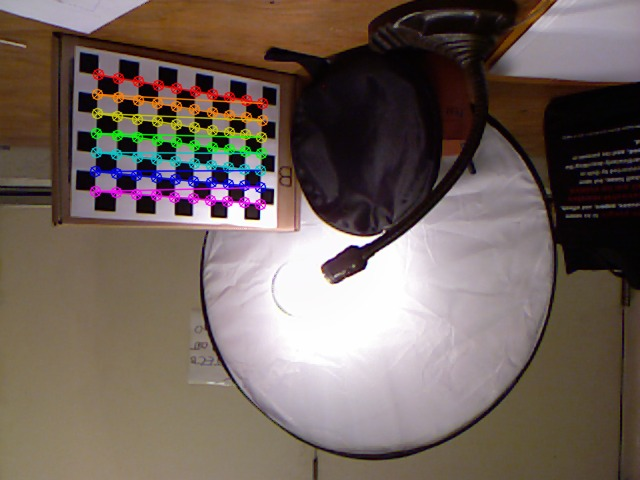
\includegraphics[width=1.7in]{ch4/diagrams/corners01.jpg} 
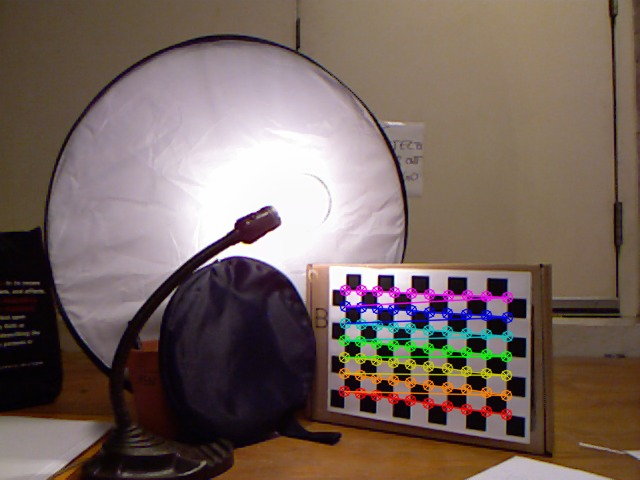
\includegraphics[width=1.7in]{ch4/diagrams/corners02.jpg} \\
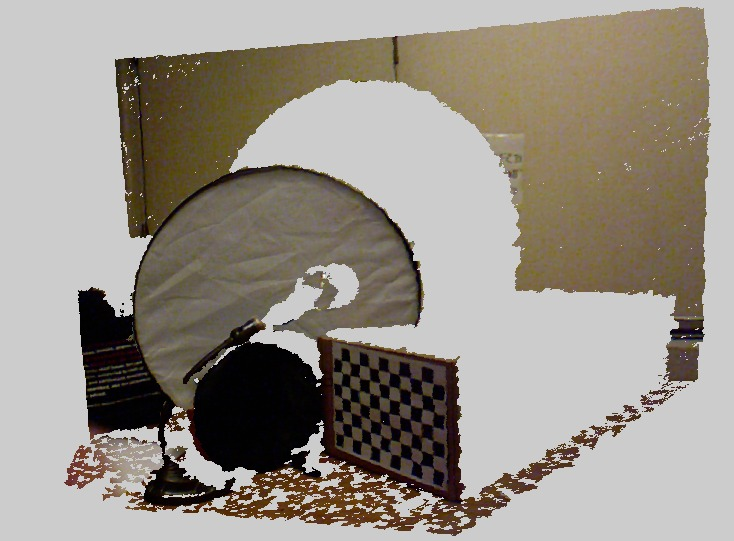
\includegraphics[width=1.7in]{ch4/diagrams/calibration_camera1.jpg} 
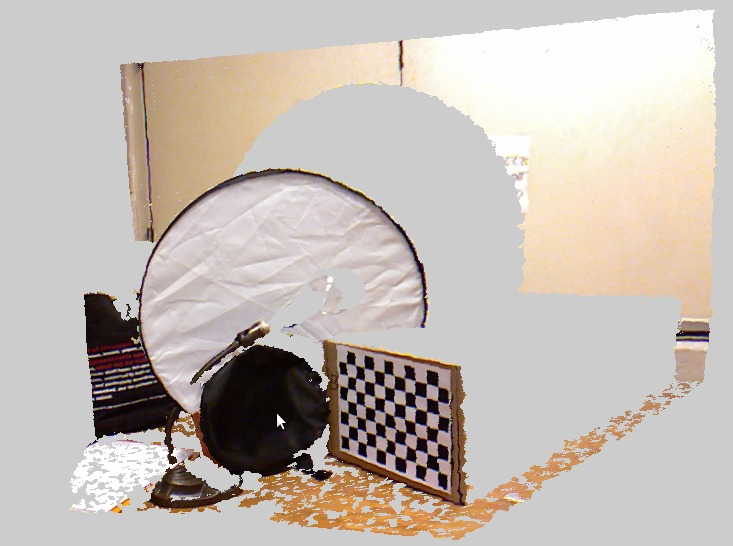
\includegraphics[width=1.7in]{ch4/diagrams/calibration_camera2.jpg} \\
%Camera Configuration and virtual cameras
\caption{Camera calibration and 3D projection of the point cloud data in world coordinate. Notice that with our setup one camera is upside down and the camera calibration is affected by the orientation and perspective difference. The corners from the checkerboard are used for the estimation of the $[\mathbf{R}_{ij}~\mathbf{t}_{ij}]$ in the camera calibration step. The images in the second row are the projection of the point cloud data from two separate Kinect cameras $C_{1}$ and $C_{2}$ onto the virtual camera $V$, and rendered with OpenGL. Notice that with our configuration the Kinects can capture differently exposed images at the same time, and th}
\label{fig_reproject}
\label{sec_sim_hdr_mul_kinect}
\end{figure}
In contrast to the typical HDR composition algorithm where the composition is performed on two images from the same image plane, we propose an algorithm that operates on the 3D data from the Kinect that are captured from two different perspective simultaneously. That is, instead of only concerning about the tonal information, we have additional spatial parameters that would be considered in the HDR composition process.  One key advantage of this approach is that we can capture simultaneously which reduces the registration problem due to camera, or in frame motions. Furthermore, this allows us to capture 3DHDR real-time (30 FPS) video of the scene. However, there are several trade offs in this approach and these limitations are discussed in Section~\ref{sec_discussion}.

\subsection{3D Image Registration}
The Kinect camera provides us a 3D measure of the scene. We can register the point cloud data $\mathbf{\tilde{M}}_{i}$ and $\mathbf{\tilde{N}}_{j}$
 from the differently exposed RGB images by projecting the cameras $Ci$ to $Cj$ and vice-versa based on their geometric relations estimated in the camera calibration process.

In Equation~\ref{eq_3D_rgb_lookup}, we described the image registration for obtaining the RGB image from the depth map on a Kinect. Similarly, we can extend such a mapping by first transforming the $j$th Kinect to the $i$th Kinect's coordinates and then obtain the RGB value from the $i$th Kinect's color camera 
\begin{equation}
\begin{split}
[u_i'~v_i'~1]^T &=  \mathbf{A}_{ci}[\mathbf{R}_i~\mathbf{t}_i][\mathbf{R}_{ji}~\mathbf{t}_{ji}]\mathbf{N}_j\\
[r_i, g_i, b_i, k_i]^T &= \mathbf{I}(u_i', v_i').
\label{eq_3D_rgb_lookup_ir}
\end{split}
\end{equation}

Now, for each $\mathbf{\tilde{M}}_{i}$ and $\mathbf{\tilde{N}}_{i}$ we have found a corresponding pair $[r_i, g_i, b_i, k_i]$ and $[r_j, g_j, b_j, k_j]$ for the HDR composition step.  Following the steps described in Section~\ref{sec_single_kinect}, we can compose an HDR image as if the color images were captured from the same camera as shown in Fig.~\ref{fig_reproject}.

\subsection{3D Point Cloud Merging}
\begin{figure}
\centering
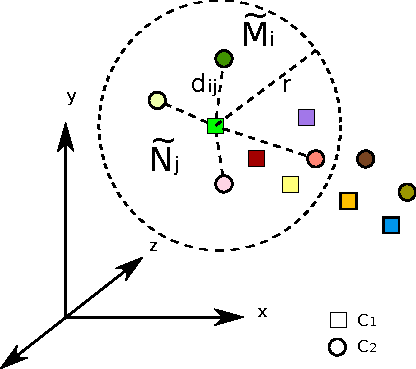
\includegraphics[width=3.3in]{ch4/diagrams/3d_data_structure.pdf} \\
%Camera Configuration and virtual cameras
\caption{Compositing of the point cloud data $\mathbf{\tilde{M}}_i$ and $\mathbf{\tilde{N}}_j$ in 3D space. The point cloud data from each Kinect are projected onto the real-world coordinates and merged based on the tonal and spatial information in (\ref{eq_match_3d_point}). $d_{ij}$ is the distance between two point cloud data in meter and $r$ is the search radius.}
\label{fig_3D_structure}
\end{figure}
The approach discussed in Section~\ref{sec_sim_hdr_mul_kinect} suggested that we could perform 3D composition of the RGB data by re-projecting the cameras onto the same image plane. Instead, we can operate directly on the point cloud data and merge the data directly in 3D space.

Given two point cloud data sets  $\mathbf{\tilde{M}_{i}}$ and $\mathbf{\tilde{N}_{j}}$ where $i$, $j$ are the index for the $i$th and the $j$th point in space, we compute their new correspondence set by finding the candidate with the best score in the similarities metrics 
\begin{equation}
\label{eq_match_3d_point} 
\begin{split}
I(i,j) &= (w_{ij}\mathbf{d}_{ij} + c_{ij}\mathbf{l}_{ij})/(w_{ij} + c{ij}), \\
\mathbf{d}_{ij} &= || \mathbf{X}_i - \mathbf{X}_j ||, \\
\mathbf{l}_{ij} &= ||{k_i\mathbf{Q}(r_i,g_i,b_i)-k_j\mathbf{Q}(r_j,g_j,b_j)}||
\end{split}
\end{equation}
where $\mathbf{X}=[X, Y, Z]$ is the position in the real-world coordinates, $\mathbf{Q}(r,g,b)$ is the light quantity vector $[f^{-1}(r), f^{-1}(g), f^{-1}(b)]^T$ based on the camera response function, $k_i$ and $k_j$ are the exposure values, and $w_{ij}$ and $c_{ij}$ are weight functions on the spatial and tonal data. 
The weighted functions can be defined as a penalty on the uncertainties in the point cloud data 
\begin{equation}
\begin{split}
c_{ij} &= s_c \\
w_{ij} &= s_d/(e(Z_i) + e(Z_j))
\end{split}
\end{equation}
where $c$ and $e$ are the certainty function of the depth map and the color image, and $s_d$ and $s_c$ is a scaling variable for the weight.

To reduce the complexity of the matching process, a k-d tree data structure is used for the search for potential candidates in close proximity. For data points that have no matches, perhaps due to shadows, or `holes' in the depth map, we simply add those data to the final result by remapping the $[r, g, b]$ into light vectors $[q_r, q_g, q_b]$. 

%\begin{figure}
%\centering
%\includegraphics[width=1.5in]{ch4/diagrams/hdr_3d_algorithm.pdf} \\
%%Camera Configuration and virtual cameras
%\caption{The tonal information  }
%\label{fig_3D_vectors}
%\end{figure}
%Lambertian model

%\section{Proposed Setup}
%why do we setup the kinects in such way, and what are the disadvantages and advantages of using multiple kinect for such setup.
%2x rgb 2x ir at different exposures
%can capture both stream at the same time, useful for video recording, and adding 

%how do we generate a high dynamic range image with the point cloud of different exposure.
%i.e., converting the rgbd (8 bits, 8 bits, 8 bits, 32 bits) to rgb (32 bits, 32 bits, 32 bits, 32 bits) and adding a vector that describe the lighting etc...
%show the math behind these algorithms (i.e., HDR composite, and ray tracing, the geometry problem and what we are solving)


\section{Results}
We successfully created an array of Kinect cameras, to capture differently exposed 3D data. In one example, using two Kinect cameras, where one is fitted with a neutral density filter, we obtained two simultaneously captured yet differently-exposed 3D sensing videos of the same subject matter.  We have tested the resulting 3DHDR camera on scenes with light shining directly into the camera. In particular, in the worst-case scenario, namely a tungsten light bulb that emits light in both visible spectrum and infrared spectrum, which was placed directly in the scene with no lamp shade, our 3DHDR camera produced excellent results, even though the individual 3D cameras failed. 

\subsection{Wearable HDR 3D Digital Eye Glass}
Our results suggested that by applying high dynamic range imaging technique to both spatial and tonal domain, we can achieve more robust tracking system and seeing aid in everyday use. To verify the feasibility of the system, we created an unique wearable 3DHDR eyeglasses prototype for everyday use. In Fig.~\ref{fig_wearable_glass}, a functional prototype which utilizes the PrimeSense 3D range sensing camera (the same technology that is used in Kinect camera) and the EPSON Moverio head mounted display is shown. The prototype allows us to further explore the use of HDR imaging with 3D camera sensors in different scenarios. For example, the wearable setup allows users to see an aug-mediated reality system which rendered the high dynamic range 3D information from the POE (point of eye) of the wearer as shown in Fig.~\ref{fig_3D_HDR_results}).


%
%\begin{subfigure}[t]{.5\textwidth}
%\centering
%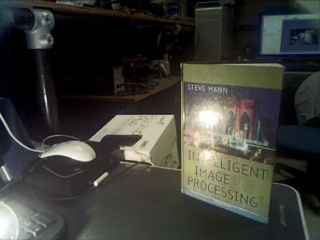
\includegraphics[width=2.3in]{ch4/diagrams/hdr_results/hdr2.jpg}
%\label{hdr_result}
%\caption{HDR Result}
%\end{subfigure}
%
%\begin{subfigure}{.5\textwidth}
%\centering
%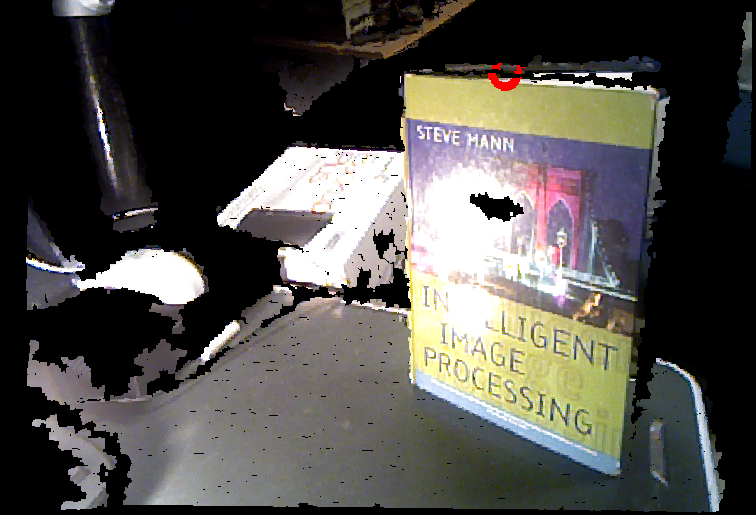
\includegraphics[width=2.3in]{ch4/diagrams/hdr_results/no_hdr.jpg}
%\label{hdr_result1}
%\caption{3D Reconstruction}
%\end{subfigure}
%
%\begin{subfigure}{.5\textwidth}
%\centering
%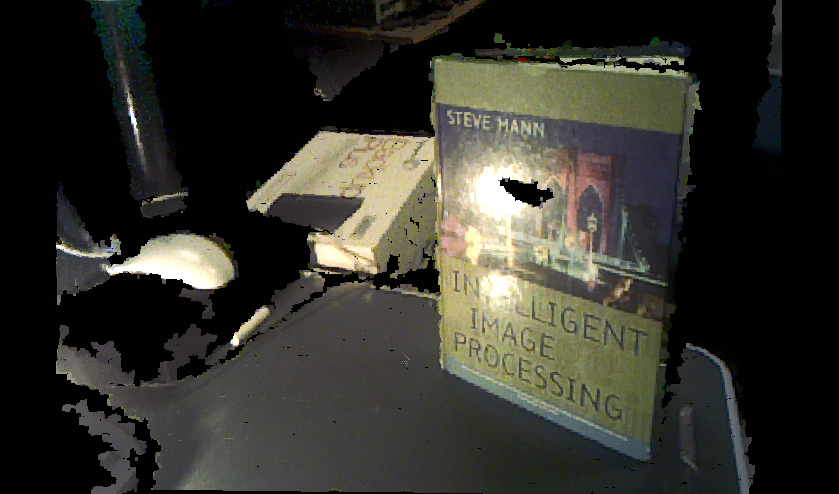
\includegraphics[width=2.3in]{ch4/diagrams/hdr_results/hdr.jpg}
%\label{hdr_result2}
%\caption{Our proposed HDR result rendered in 3D}
%\end{subfigure}

\begin{figure*}[t!]
    \centering
    \begin{subfigure}{0.32\textwidth}
        \centering
        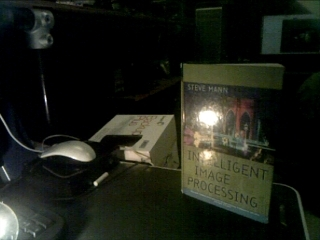
\includegraphics[height=1.4in]{ch4/diagrams/hdr_results/low.jpg}
        \caption{Lower Exposure}
        \label{hdr_low_expos}
    \end{subfigure}%
    ~ 
    \begin{subfigure}{0.32\textwidth}
        \centering
        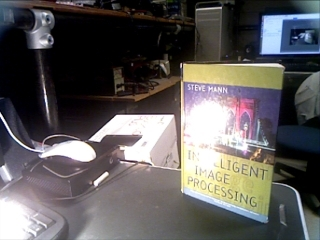
\includegraphics[height=1.4in]{ch4/diagrams/hdr_results/high.jpg}
        \caption{Higher Exposure}
        \label{hdr_high_expos}
    \end{subfigure}
    ~
    \begin{subfigure}{0.32\textwidth}
        \centering
        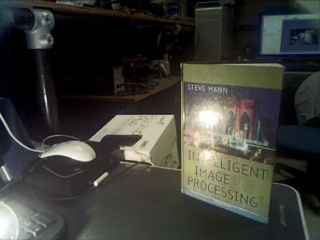
\includegraphics[height=1.4in]{ch4/diagrams/hdr_results/hdr2.jpg}
        \caption{HDR Result}
        \label{hdr_result}
    \end{subfigure}
    \centering
    \begin{subfigure}{0.4\textwidth}
        \centering
        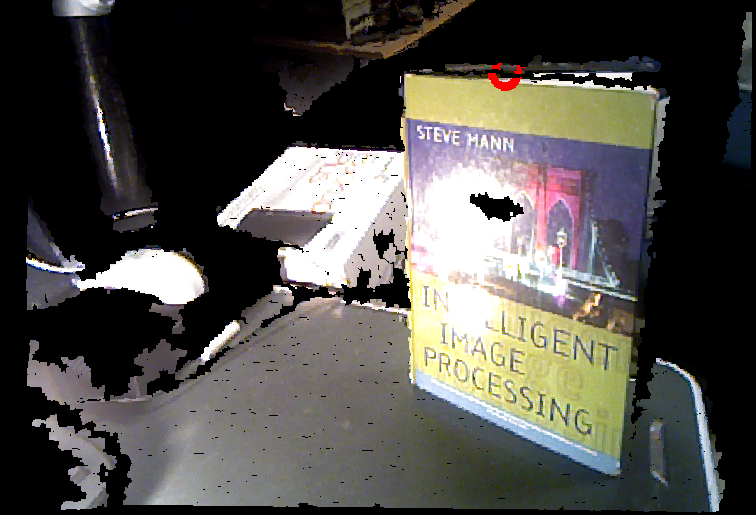
\includegraphics[height=1.8in]{ch4/diagrams/hdr_results/no_hdr.jpg}
        \caption{3D Reconstruction}
        \label{hdr_result1}
    \end{subfigure}
    ~
    \begin{subfigure}{0.55\textwidth}
	\centering	
	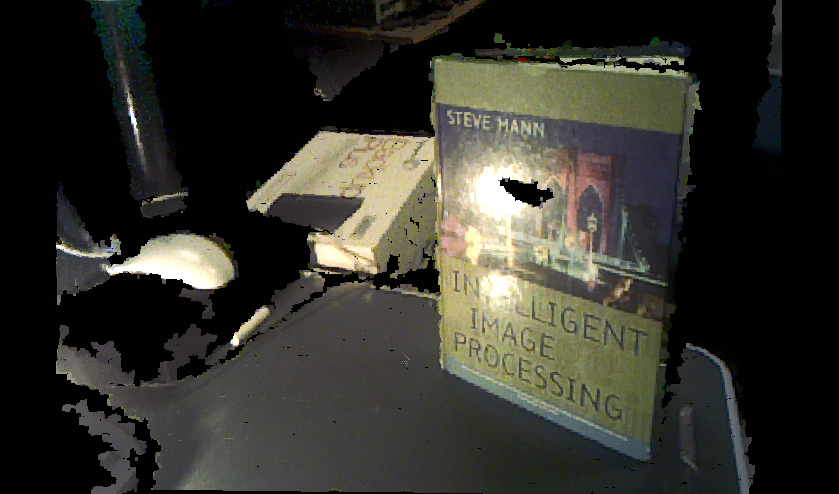
\includegraphics[height=1.8in]{ch4/diagrams/hdr_results/hdr.jpg}
	\caption{Our proposed HDR result rendered in 3D}
	\label{hdr_result2}
    \end{subfigure}
    
    \caption{Example of our 3DHDR rendering for wearable eyeglasses. Notice that the low exposure image captures the detail of the book cover but unable to capture the background. On the other hand, the high exposure image captures the background image but the highlight detail of surfaces such as the book cover and the mouse on the desk are saturated. By combining the images and the depth maps, we reconstruct a 3D reconstruction of the scene from a virtual camera. By projecting the scene onto wearer's POE, we can reconstruct a scene from the same perspective as how the users may see in real life.}
\label{fig_3D_HDR_results}
\end{figure*}

\section{Discussion}
\label{sec_discussion}
This chapter proposed a method to reconstruct 3DHDR scene using one or more Kinect. However, there are several trade offs we shall consider in our proposed configuration. Particularly, there are some key limitations shall be addressed in the future work in order to produce high quality 3DHDR videos for everyday use.

\subsubsection{Interference among Kinects}
The Kinect uses a structured light pattern to reconstruct 3D data from the scene with the help from an IR laser projector. When multiple Kinects are used in the same space, there are interferences that would reduce the accuracy of the depth measure. Several approaches had been proposed to reduce such problem (e.g., \cite{maimone2012reducing}). One solution is to combine different 3D sensing technology such as time-of-flight 3D sensor (e.g., SoftKinetic) to reduce the interference between the sensors. 

\subsubsection{Programmable 3D cameras}
Unfortunately, the current Kinect does not provide fine grain control over the exposure settings and thus an ND filter is required for our setup. In addition, Kinect sensor does not provide hardware support in synchronizing the data streams, and thus we still suffer a minor latency issue. 

\subsubsection{High Resolution and High Accuracy Depth Sensor}
One leading limiting factor for the reconstruction stage is the spatial resolution and noise performance of the 3D sensors. In the future, a higher resolution depth map will significantly improve the overall accuracy and the quality of the output.

\subsubsection{Noise Modeling and Filtering}
Lastly, to improve the results we can employ various noise reduction algorithms for both the image and depth map image. Particularly, the depth map often shows missing data (e.g., holes and shadows) in the scene, as shown in Fig.~\ref{fig_3D_HDR_results}. These can be addressed by applying spatial and temporal filters \cite{matyunin2011temporal} on the depth map stream to improve our final results.

\section{Social Implications}
One of the applications of our 3DHDR system is wearable computing.
An HDR camera system, in general, enables the user to capture a wider variety
of scenes than a regular camera which can only capture LDR scenes. That is,
an HDR camera system can see into dark and bright area of scenes `better' than
conventional cameras. Therefore, a wearable 3DHDR EyeTap wearable computing
device can act as a vision aid - enhancing and protecting the viewers vision.
For example, through an HDR camera system, a user can look into the headlights
of a car in a dark alley and still see the license plate and the driver's face.
A user can also safely view welding
which would otherwise be harmful to the naked eye~\cite{mann2012hdrchitecture}.%
%However, if this is used in a wearable system, it is possible that, with prolonged use, the user's eyes will lose some of their natural dynamic range over time due to the lack of viewing high dynamic scenes with their naked eyes (need reference).

The 3DHDR system used in this fashion, as a vision aid in a wearable computing platform, can be classified as a sousveillance system \cite{mann2004sousveillance,mann2006cyborglogging,mann2002sousveillance}, that is, instead of a camera system mounted on a building, which is surveillance, the camera is
human-centric and the world through this device is captured as a first person
view. In the past several decades and in present times, there have been
a number of debates in the mass media over the appropriate use of sousveillance
devices, such as wearable camera systems. On one hand, sousveillance devices are viewed as
a deprivation of personal privacy that should be forbidden in any public area.
On the other hand, others view such devices as a revolutionary personal
assistance that can act as a visual aid and perform augmented and (aug)mediated
reality \cite{hill2004reality} tasks, such as providing an interactive
augmented/augmediated reality interactions on subject matter in view of a
user as the user sees it in a first-person view \cite{aimone2003eyetap}.

As a vision aid, it is impractical for it to be forbidden, as those forbidding
it will assume liability for any side effects of non-usage (e.g. if a person
trips and falls because they were required to not wear their DEG).
Moreover, sousveillance may provide a necessary
balance-of-power between the authorities and individuals.

\section{Conclusion}
We successfully demonstrated a 3DHDR camera constructed from two
Kinect sensors, one of which was fitted with a neutral density filter.
The resulting differently exposed (one darker and one lighter) data streams
were merged in 3D to compensate for the parallax induced by the cameras
being in slightly different positions.

We were able to capture 3D information from high contrast scenes.
This suggests the possibility of making 3D cameras that can work in
outdoor settings or settings where lights are shining directly into
the camera. Thus it is possible to build a 3D camera that can be used for
sousveillance (e.g. wearable gesture-sensing), where the wearer does not
necessarily have control over the placement of lighting
fixtures and the like in the scene.

